% Gemini theme
% See: https://rev.cs.uchicago.edu/k4rtik/gemini-uccs
% A fork of https://github.com/anishathalye/gemini

\documentclass[final]{beamer}

% ====================
% Packages
% ====================
\usepackage{amsfonts}
\usepackage[T1]{fontenc}
\usepackage{lmodern}
\usepackage[size=custom,width=120,height=72,scale=1.0]{beamerposter}
\geometry{paperwidth=36in,paperheight=24in}
\usetheme{gemini}
\usecolortheme{ucf}
% ====================
% Titleless block
% ====================
\newenvironment{titlelessblock}{%
  \begin{beamercolorbox}[
    wd=\linewidth,
  ]{block body}
}{%
  \end{beamercolorbox}
}
% ====================
% Extension subtitle
% ====================
\newcommand{\extensionsubtitle}[1]{%
  \vspace{-0.5em}
  \begin{center}
    {\color{maroon}\fontsize{26}{36}\selectfont\bfseries #1}
  \end{center}

}

\usepackage{graphicx}
\usepackage{booktabs}
\usepackage{tikz}
\usepackage{pgfplots}
\usepackage{caption}
\pgfplotsset{compat=1.17}
\usepackage{setspace}

% ====================
% Lengths
% ====================

% If you have N columns, choose \sepwidth and \colwidth such that
% (N+1)*\sepwidth + N*\colwidth = \paperwidth
\newlength{\sepwidth}
\newlength{\colwidth}
% Four-column layout: (4 + 1) * 0.016 + 4 * 0.23 = 1.0
\setlength{\sepwidth}{0.016\paperwidth}
\setlength{\colwidth}{0.23\paperwidth}

\newcommand{\separatorcolumn}{\begin{column}{\sepwidth}\end{column}}

% ====================
% Title
% ====================

\title{Improving Tree of Thoughts with Batching and Refinement}

\author{Minghan Gao (mg2328) \and Warren Hua (wsh48) \and Zhichun Zhang (zz547) \and Yihan Zhao (yz2788)}

% ====================
% Footer (optional)
% ====================

\footercontent{
  }
% (can be left out to remove footer)

% ====================
% Logo (optional)
% ====================

% use this to include logos on the left and/or right side of the header:
% \logoright{\includegraphics[height=7cm]{logo1.pdf}}
% \logoleft{\includegraphics[height=7cm]{logo2.pdf}}

% ====================
% Body
% ====================

\begin{document}
\addtobeamertemplate{headline}{}
{
    \begin{tikzpicture}[remember picture,overlay]
      \node [anchor=north west, inner sep=3cm] at ([xshift=0.0cm,yshift=2.5cm]current page.north west)
      {
\includegraphics[height=3cm]{logos/cornell-logo.png}}; % also try shield-white.eps
    \end{tikzpicture}
}

\begin{frame}[t]
\vspace{-0.9em}% tighten the gap between the project title bar and the first block in each column
\begin{columns}[t]
\separatorcolumn

% ============================================================
% COLUMN 1 -- Introduction (Why ToT?)
% ============================================================
\begin{column}{\colwidth}

\begin{block}{Why Tree of Thoughts?}
    \vspace{-0.em}
    \centering
    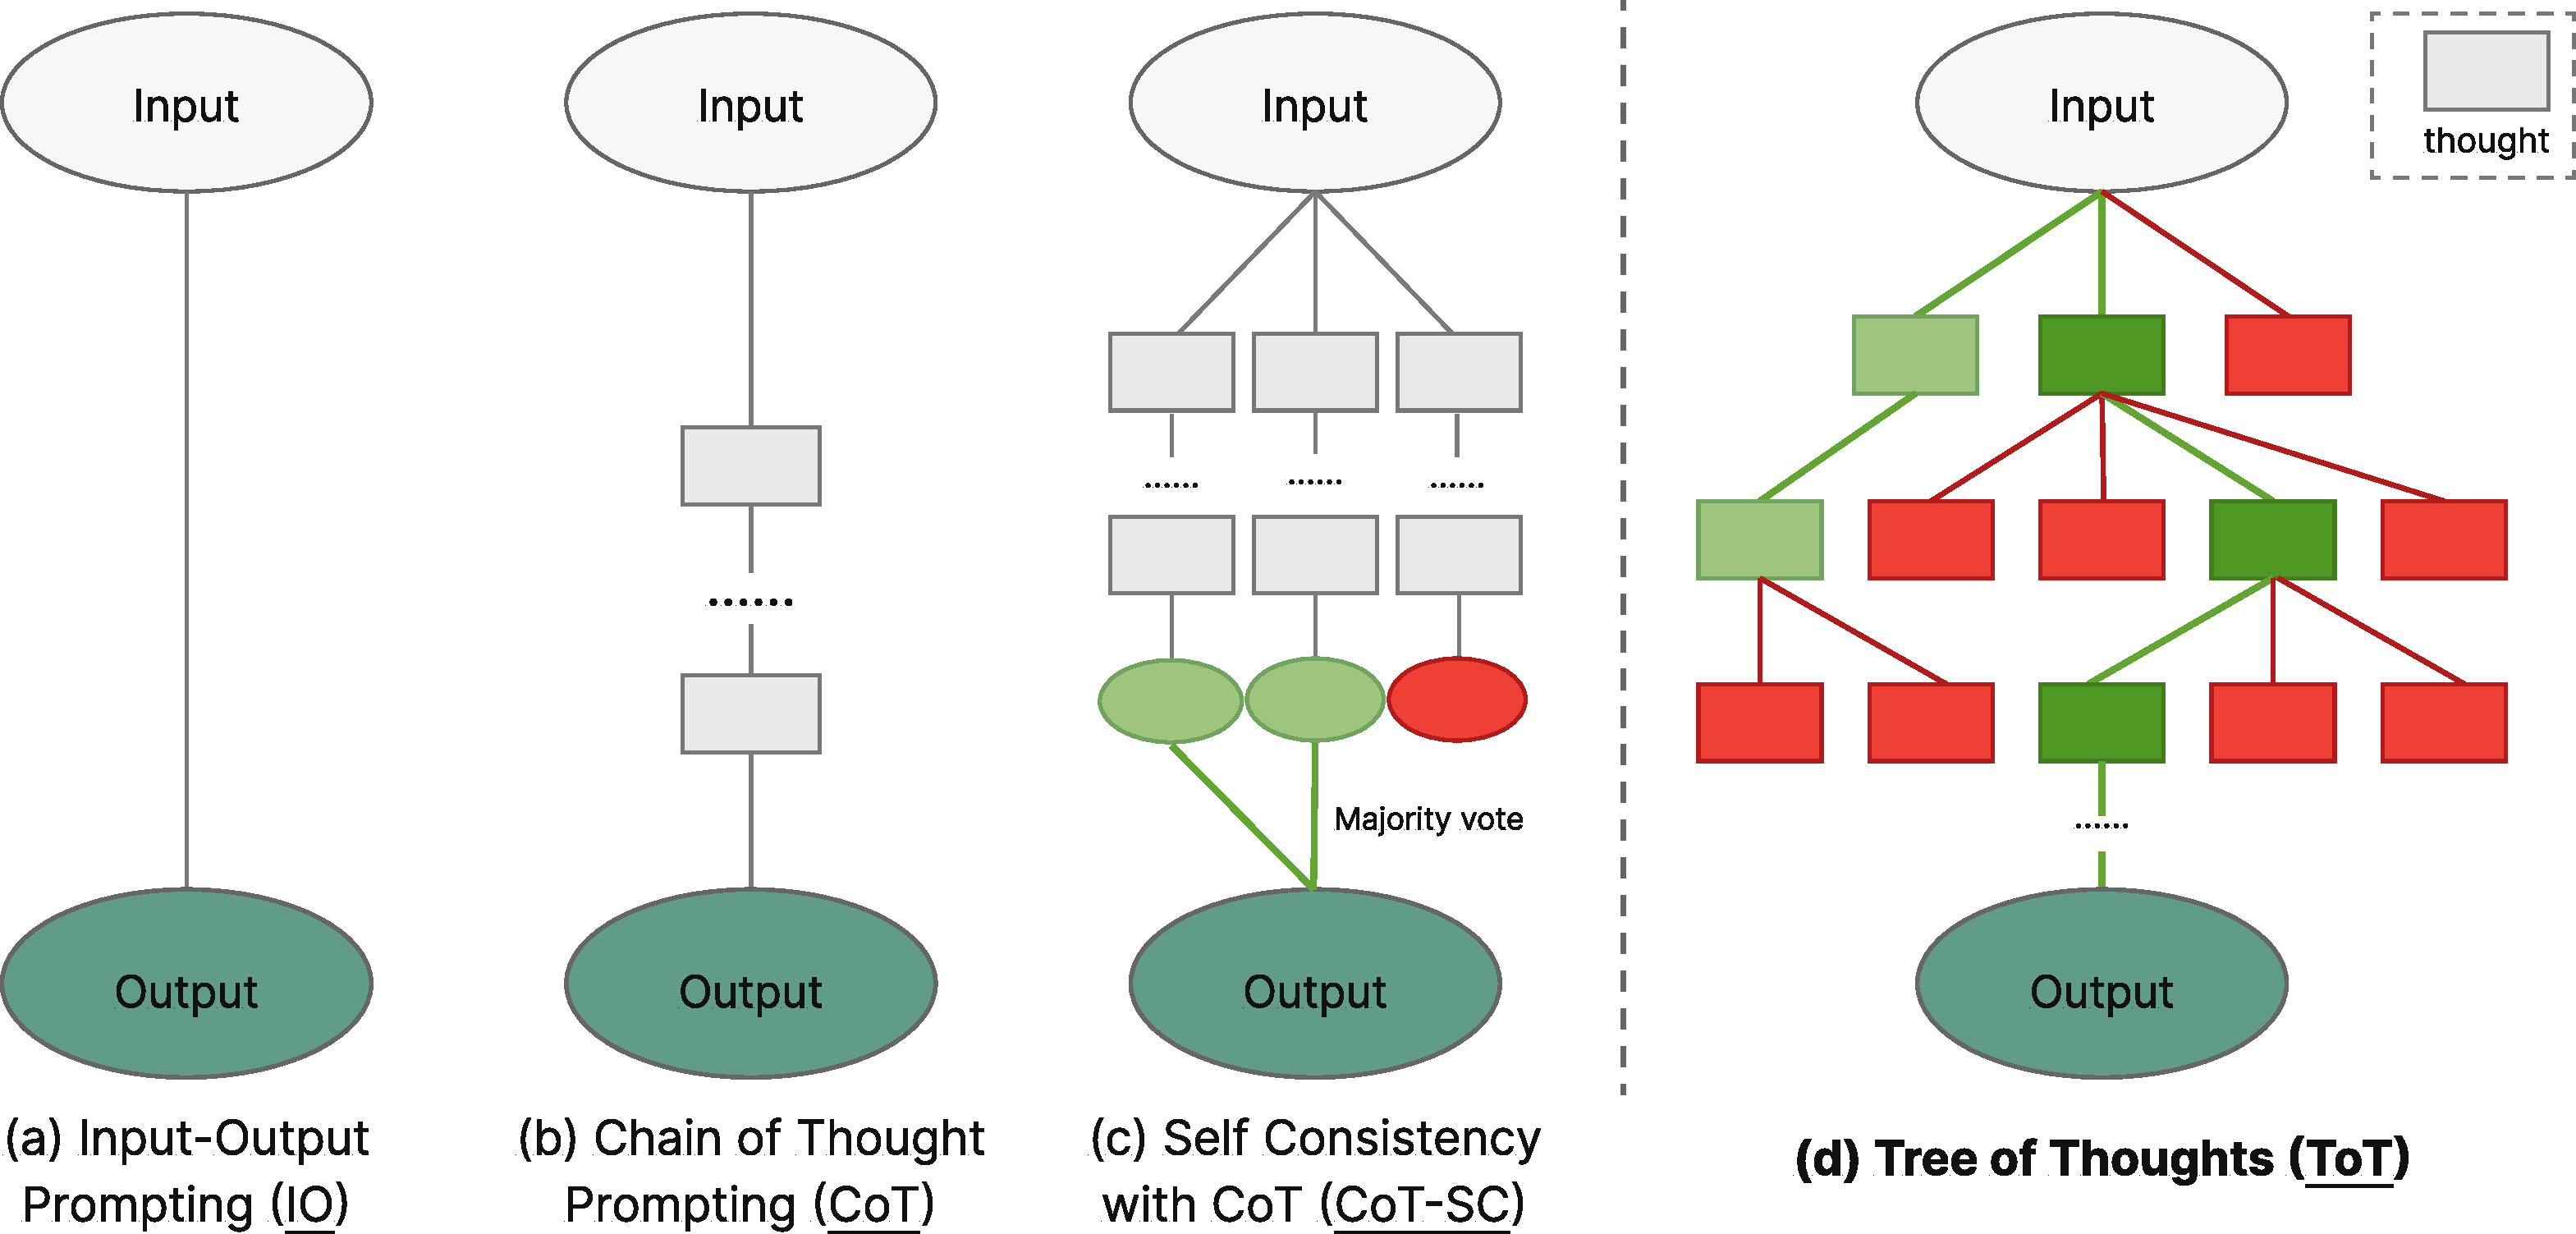
\includegraphics[width=\linewidth]{fig2.pdf}
    % \captionof{figure}{Comparison of IO, CoT, self-consistency, and Tree of Thoughts prompting.}
    \vspace{-2.2em}
    \begin{itemize}
    \item {\small \textbf{Problem:} LLMs decode one path at a time. One bad early step ruins the final answer.}

    \item {\small \textbf{Paper idea:} ToT turns reasoning into a search tree: generate candidate thoughts, evaluate them, and backtrack when needed.}

    \item {\small \textbf{Our work:}}
\begin{enumerate}
    \item Reproduced ToT on Game of 24, Crosswords, and Creative Writing using modern Gemini models.
    \item Tested batched vs.\ un-batched evaluation on Game of 24 and Crosswords.
    \item Developed two remedial strategies: a zero-cost verifier tiebreaker and a half-batching scheme.
    \item Extended Creative Writing with post-generation refinement and score-based candidate selection.
\end{enumerate}
\end{itemize}
  \vspace{-1.8em}
    \noindent


\begin{figure}[h]
    \centering
    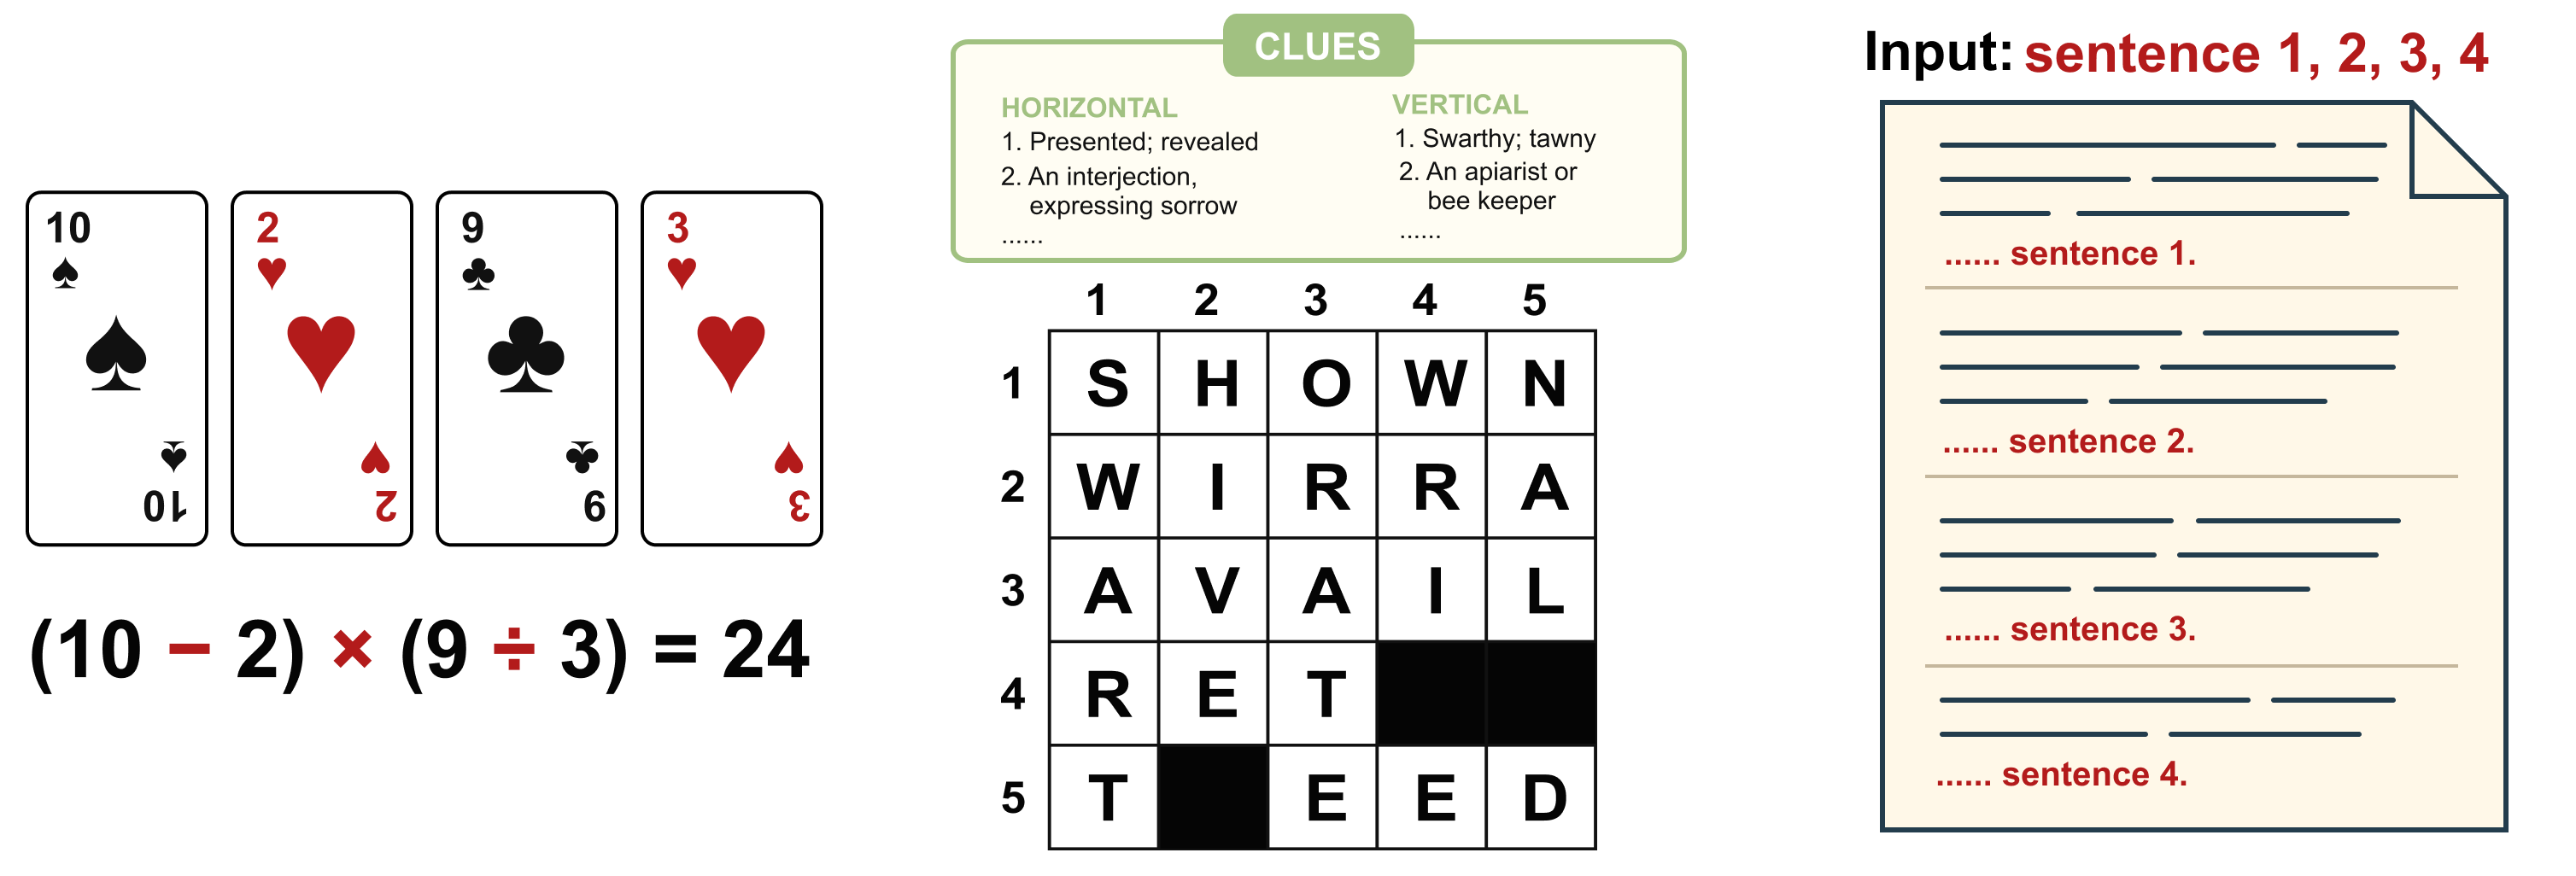
\includegraphics[width=0.9\linewidth]{tasks.png}
    \vspace{-0.7em}
\end{figure}

    
    % \begin{minipage}[t]{0.34\linewidth}
    %   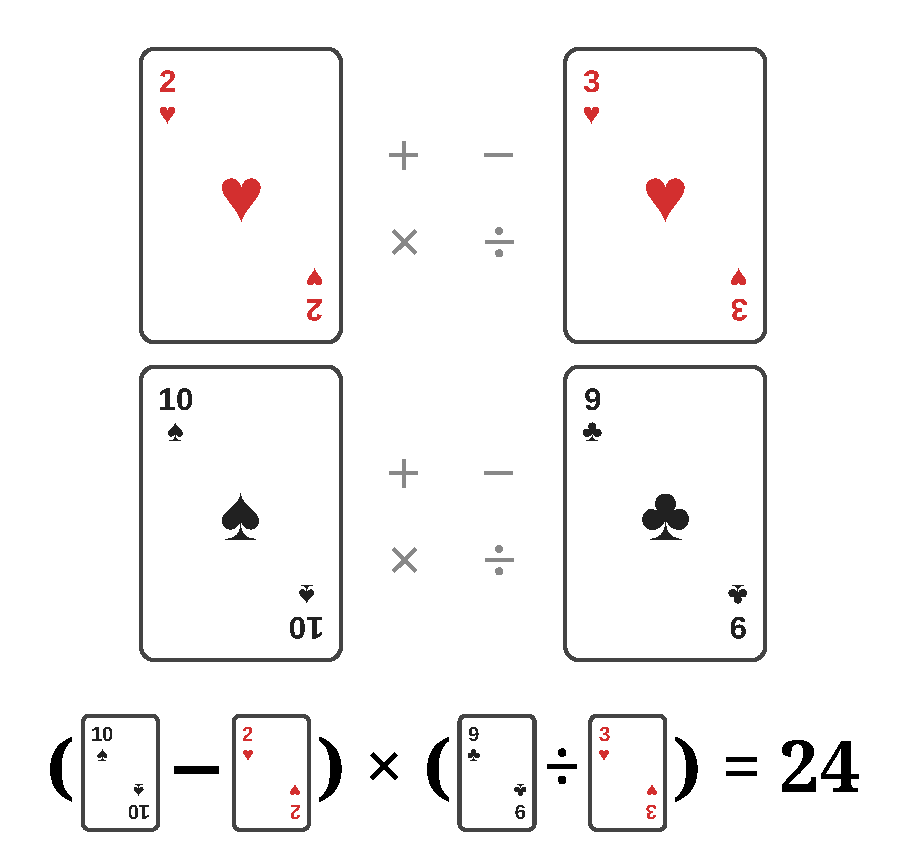
\includegraphics[width=\linewidth]{G24_plots/game_illustration.pdf}
    % \end{minipage}%
    % \hfill
    % \begin{minipage}[t]{0.33\linewidth}
    %   \includegraphics[width=\linewidth]{IMAGE2.pdf}
    % \end{minipage}%
    % \hfill
    % \begin{minipage}[t]{0.33\linewidth}
    %   
\includegraphics[width=\linewidth]{task3img.pdf}
    % \end{minipage}
\end{block}




% ============================================================
% COLUMN 3 -- Crosswords
% ============================================================

\begin{block}{Crosswords: Main Results}
\vspace{-1.3em}
\begin{figure}
  \centering
  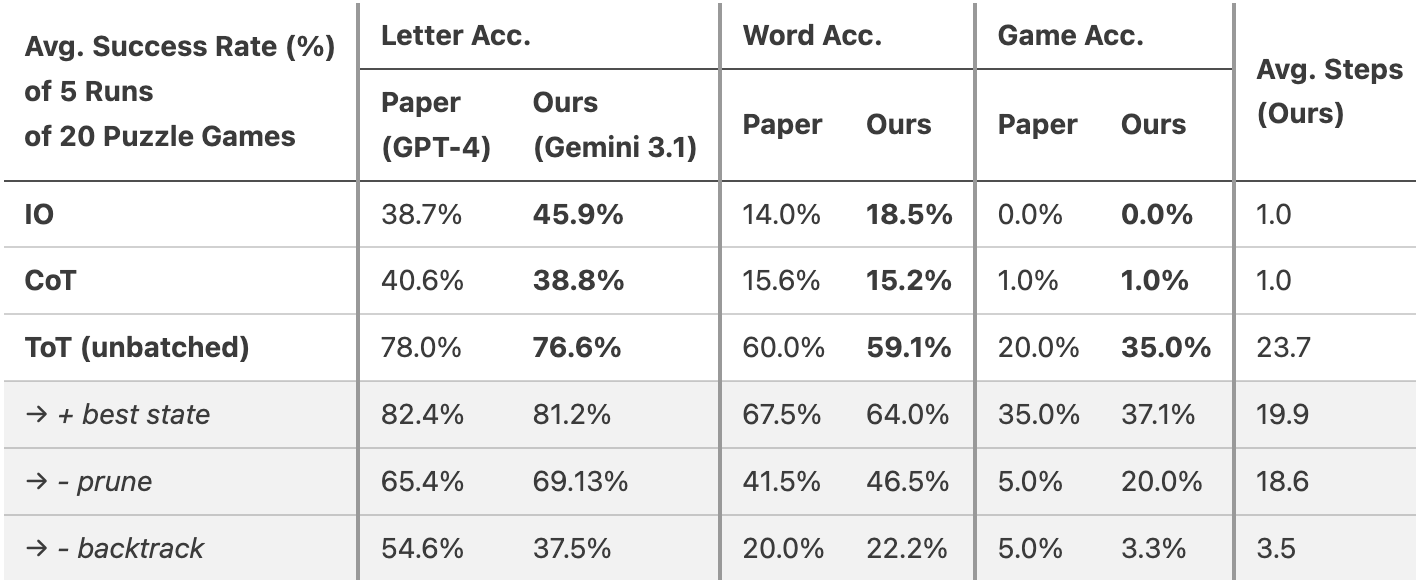
\includegraphics[width=\linewidth]{CW_plots/fig1.png}
\end{figure}

\vspace{-1em}
\begin{minipage}[t]{0.52\linewidth}
{\footnotesize \linespread{0.1}\selectfont
\textbf{1. Backtracking is the engine.} Removing backtracking makes ToT nearly greedy. \\
\textbf{2. Pruning earns its keep}. Removing pruning keeps too many weak branches.\\
\textbf{3. }Gem-3.1 outperformed GPT-4 with \textbf{stronger word-level recall and  constraint reasoning}, but still has boosts via ToT.\\
\textbf{4.  Improvement from best-state is limited:} Our DFS  commits to the right grid when it finds it. Only \textbf{14\%} had a better intermediate state than final
}
\end{minipage}
\hfill
\begin{minipage}[t]{0.45\linewidth}
    \vspace{-1em}
  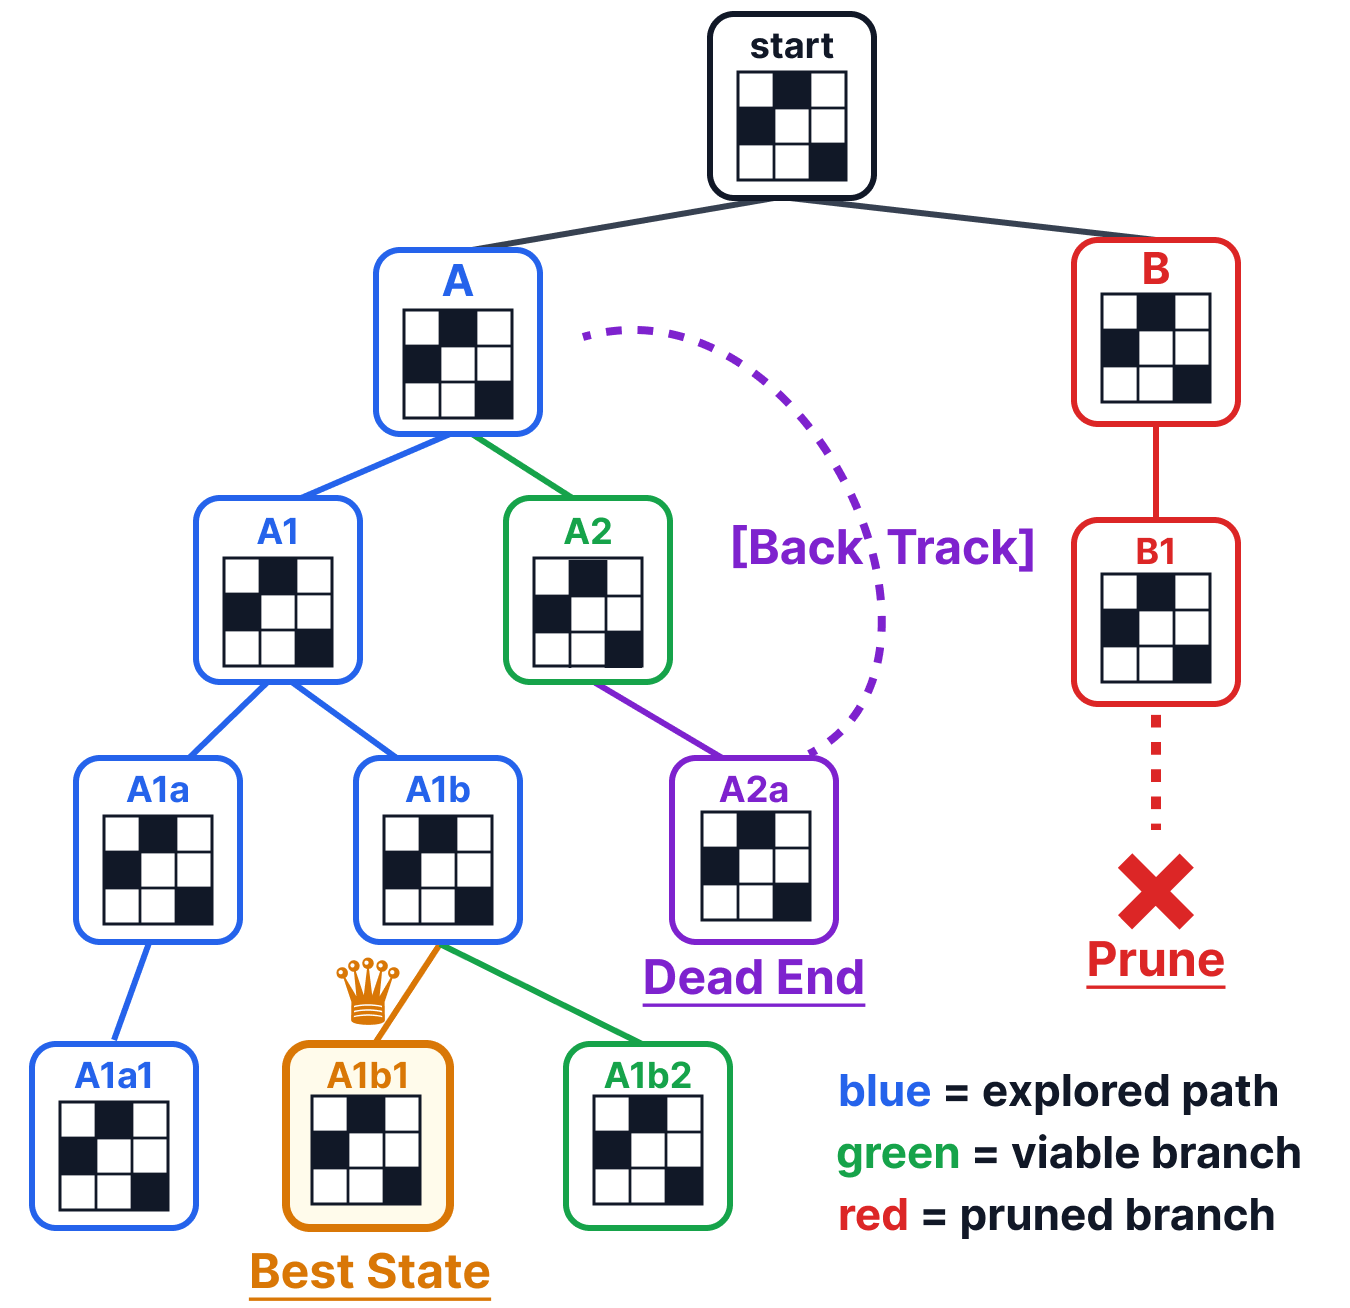
\includegraphics[width=\linewidth]{CW_plots/fig5.png}
\end{minipage}
 \end{block}


\end{column}

\separatorcolumn

\begin{column}{\colwidth}

% --- Block 2: Batching Problem ---
\begin{titlelessblock}
\vspace{-0.5em}
\extensionsubtitle{Extension: The Batching Problem}


\begin{figure}[h]
    \centering
    \vspace{-0.8em}
    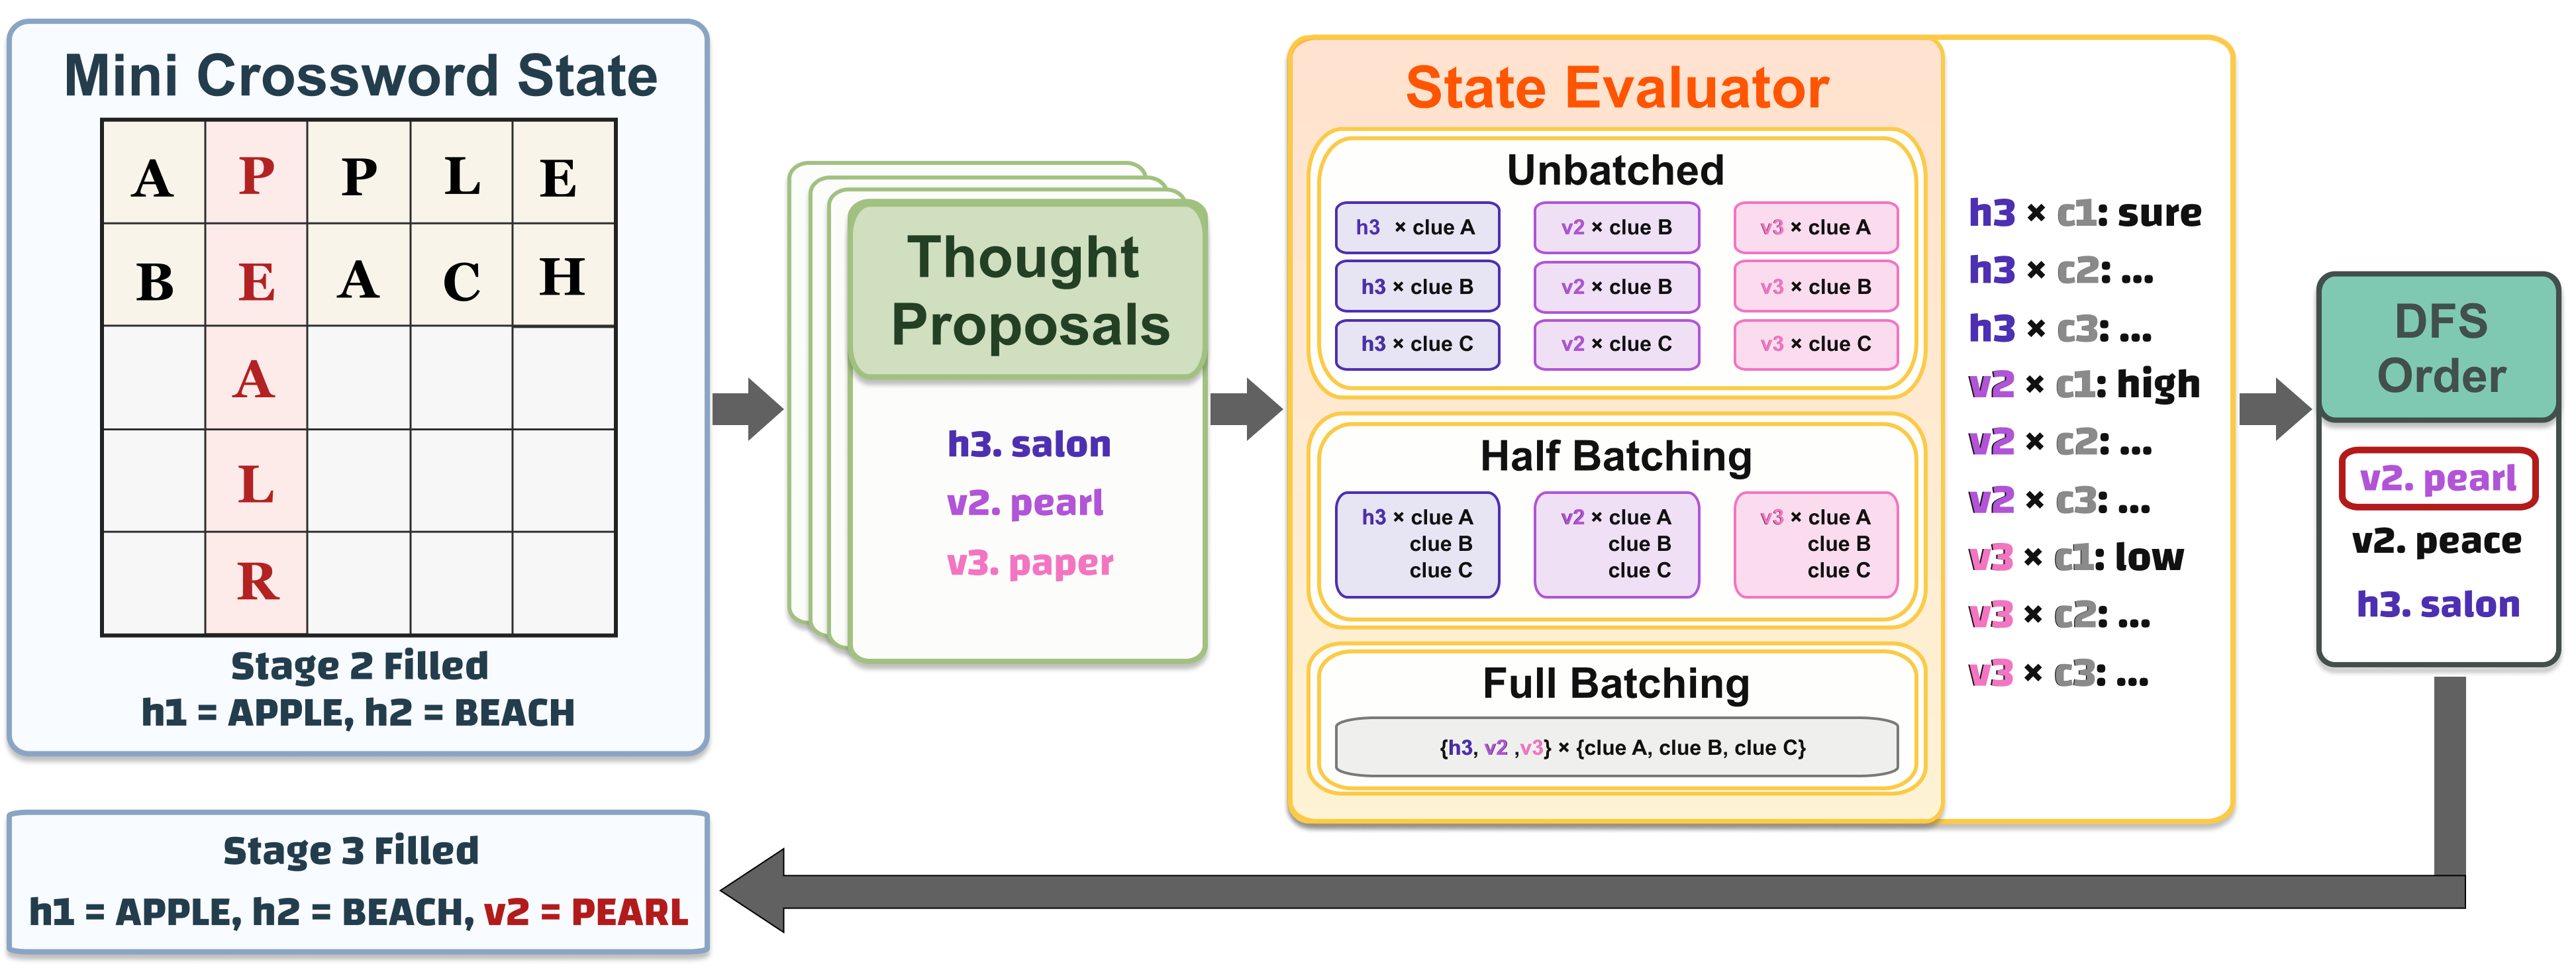
\includegraphics[width=\linewidth]{CW_plots/fig0.png}
    \vspace{-1.9em}
\end{figure}


% {\footnotesize \textbf {Original} one candidate $\times$ one clue -> 1 call \\  \textbf{Full batching} many candidates $\times$ many clues -> 1 call\\ \textbf{Half Bbtching} one candidate $\times$ multiple clues -> 1 call\\
%  }
%     \vspace{-0.4em}

\begin{figure}[h]
    \centering
    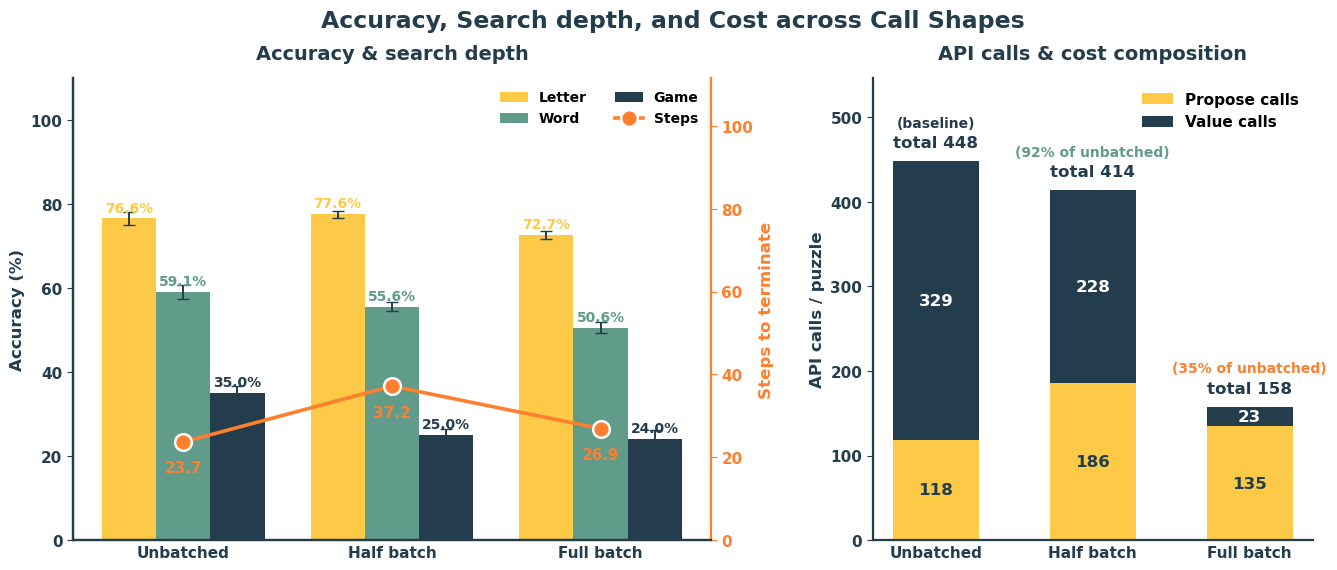
\includegraphics[width=0.9\linewidth]{CW_plots/fig2.png}
    \vspace{-1.0em}
\end{figure}


{\small\textbf{ - Full batch:}  65\% cheaper than unbatched ($158$v.s$448$ calls). The \textbf{long list noise drops game accuracy} ($35.0\%$$\rightarrow$$24.0\%$)}\\
{\small \textbf{ - Half batch:} $11\%$ cheaper than unbatched but loses $9\%$ on game acc. It is  \textbf{ most stable } one with \textbf{highest letter accuracy (77.6\%)}. It gains local context via larger average search depth (and API calls).}

\vspace{-0.3em}
% \heading{Why Batching Hurts}
\heading{Increase Accuracy for Batched Evaluator}
\vspace{-0.5em}

\begin{figure}[h]
    \centering
    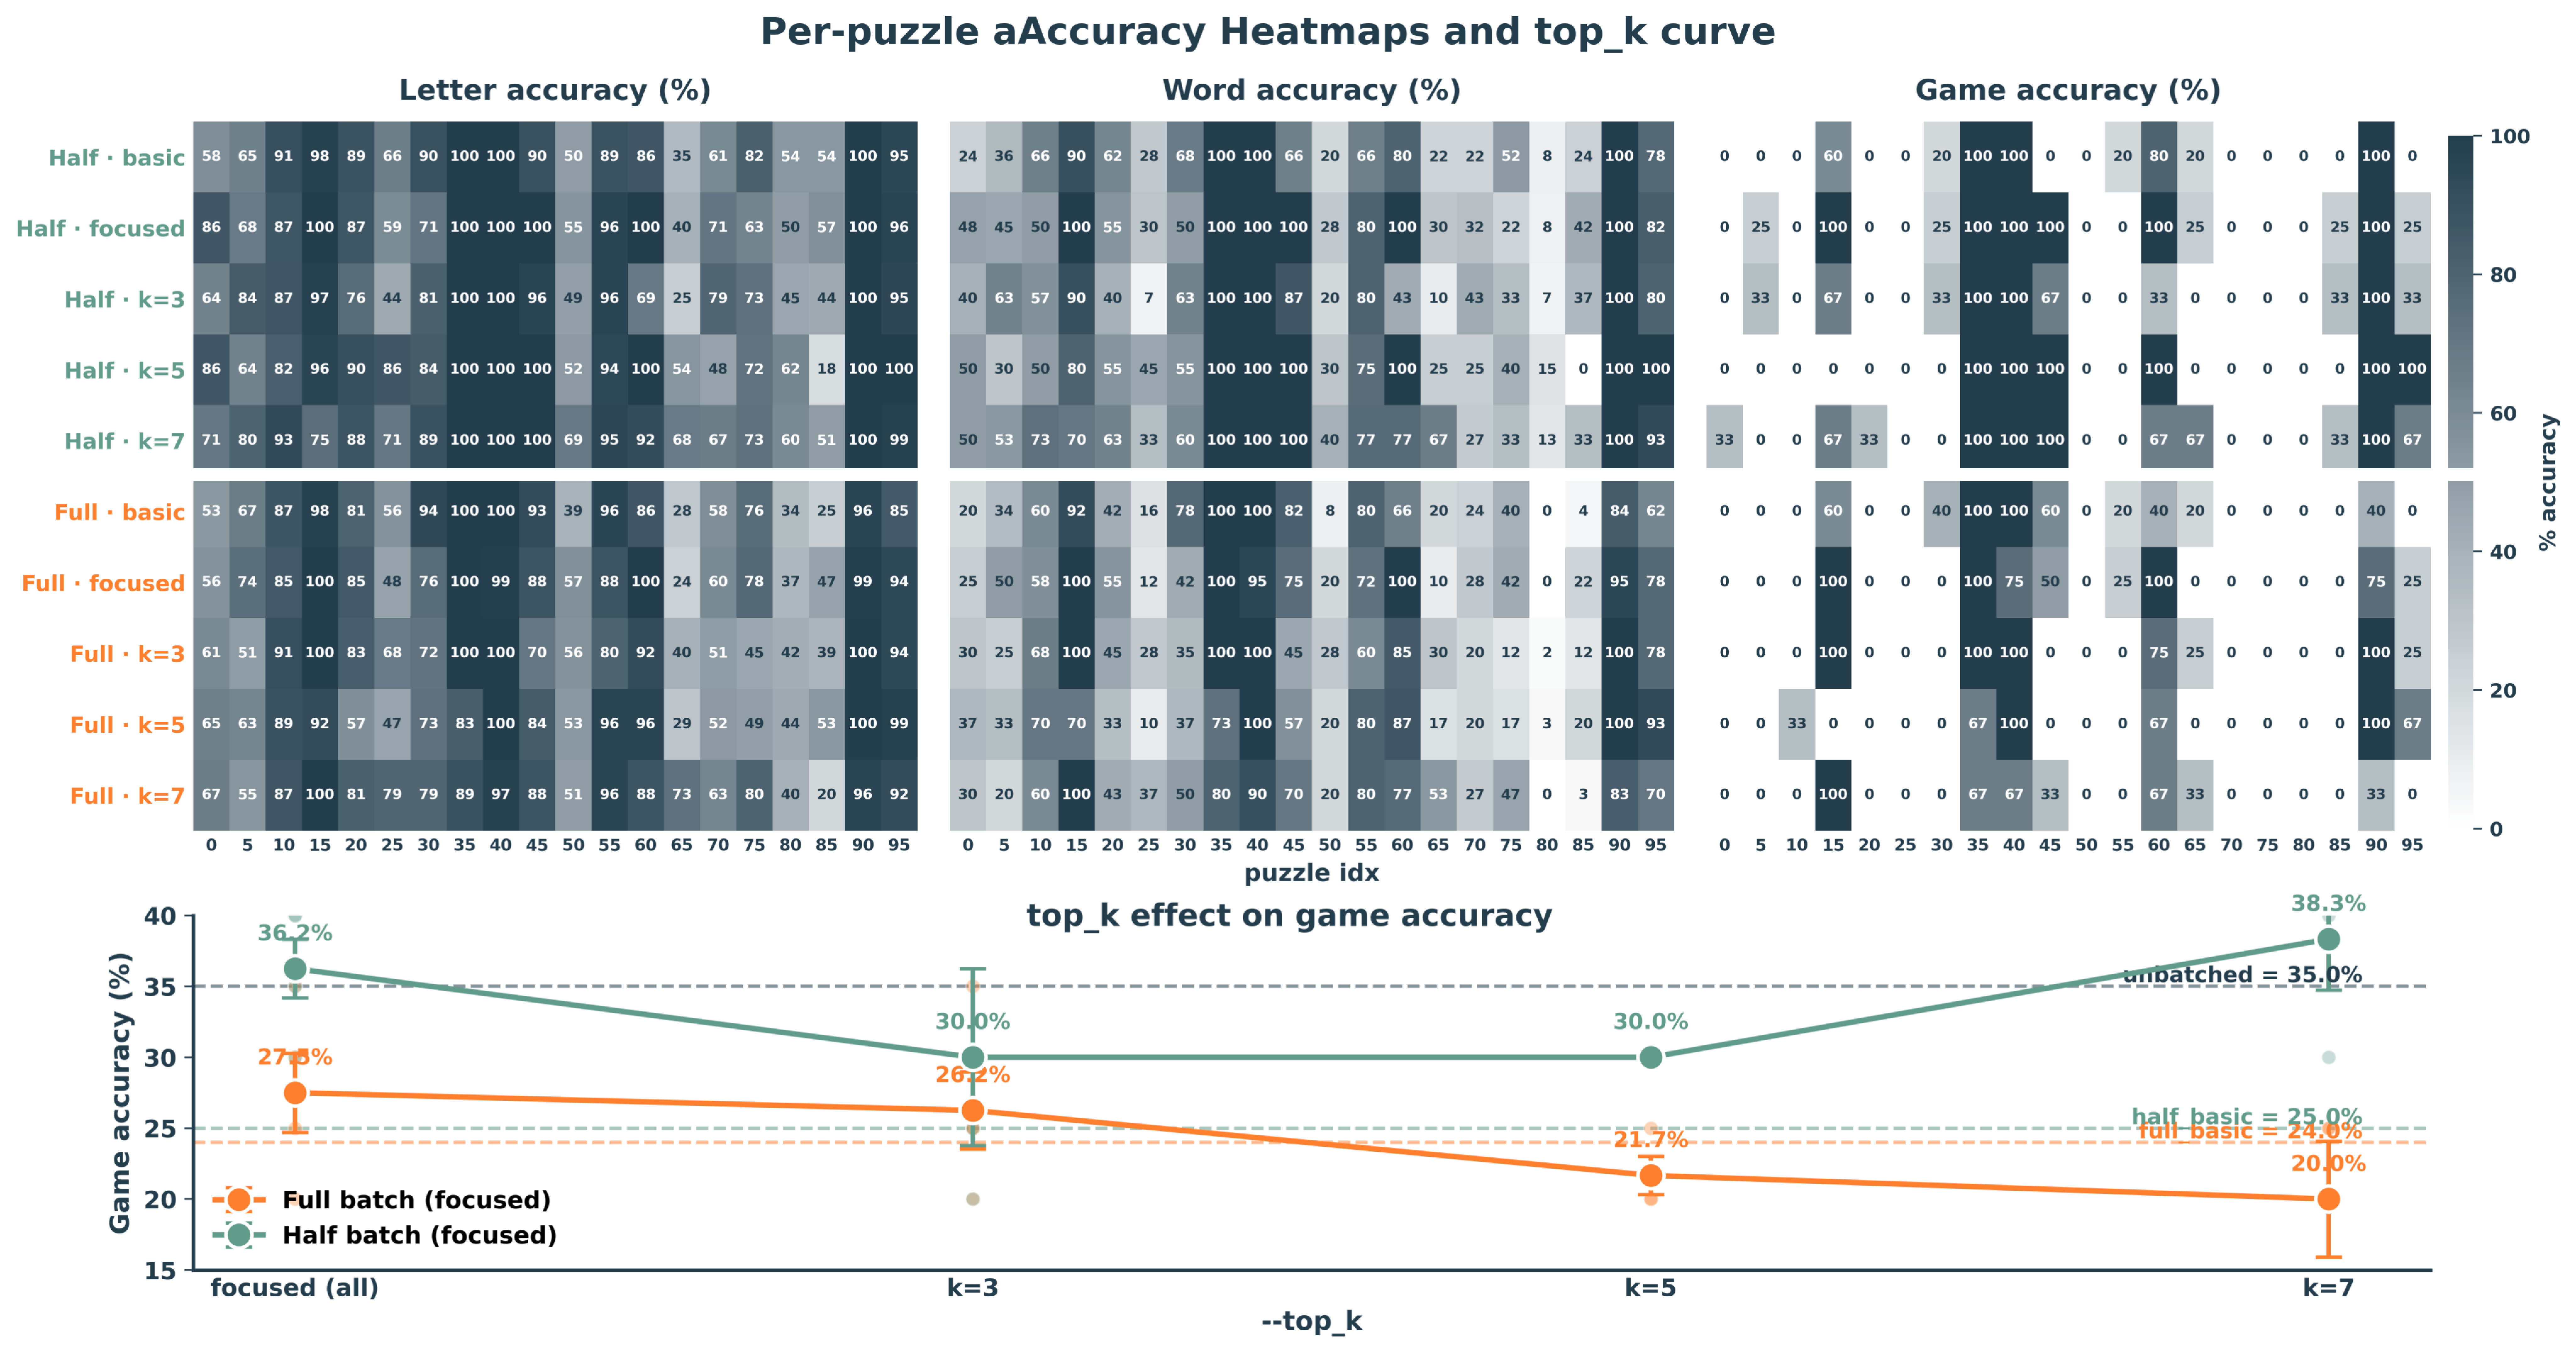
\includegraphics[width=\linewidth]{CW_plots/fig7.png}
    \vspace{-2.6em}
\end{figure}
\begin{minipage}[t]{0.52\linewidth}



{\small  \begin{itemize}
    \item \textbf{Full batch:} $top_k=0$ (all testable clues) ($27.5\%$) and $top_k=3$ ($26.2\%$) outperformed 
    \item  \textbf{Half batch: } $top_k=0 $ ($36.2\%$) and $top_k=7$ ($38.3\%$) are tied
\end{itemize}}
\vspace{-0.6em}
{\small \textbf{Focused} dominates on both batch levels. accurate$\uparrow$ and cheaper}

% {\footnotesize \selectfont
% \textbf{Focused} dominates on both batch levels: accurate$\uparrow$ and cheaper. The candidate-level question is easier.\\}
    \vspace{-0.3em}
\begin{figure}[h]
    \centering
    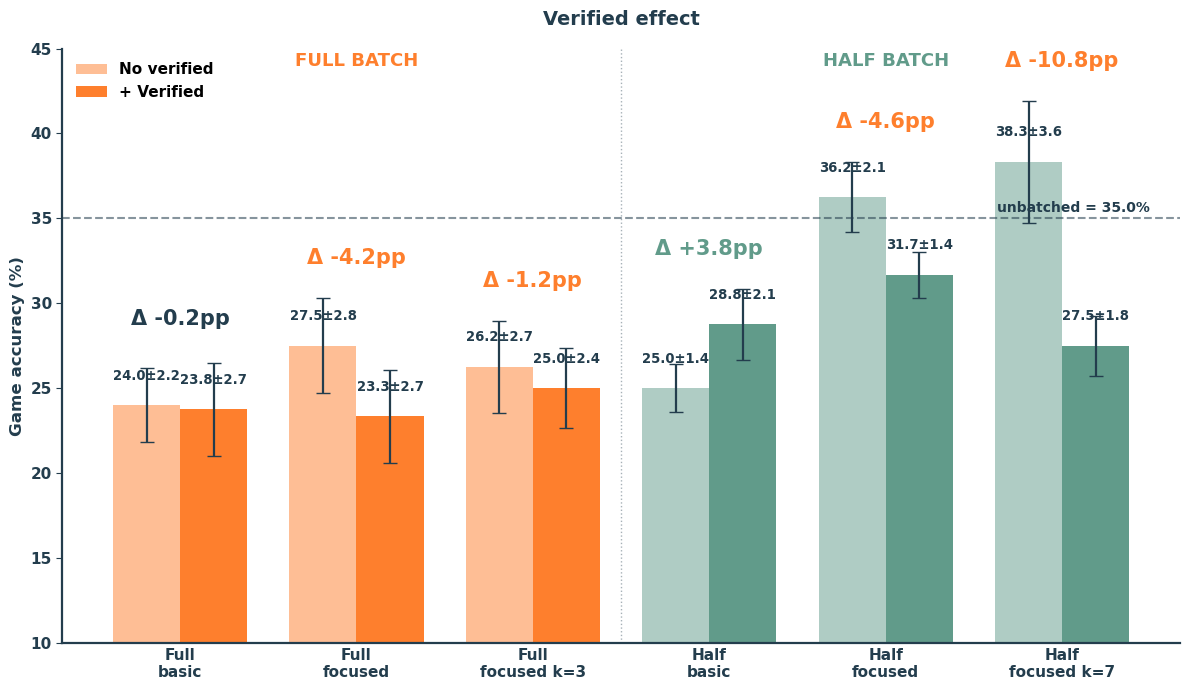
\includegraphics[width=\linewidth]{CW_plots/fig8.png}
    \vspace{-2em}
\end{figure}

{\footnotesize  \linespread{0.1}\selectfont
\textbf{Verified} itself does not reduce variance.
It is Pareto regression on "focused + verified" that most stage-1 kills get restored.
}
\end{minipage}
\hfill
\begin{minipage}[t]{0.46\linewidth}
  \vspace{0.0em}
  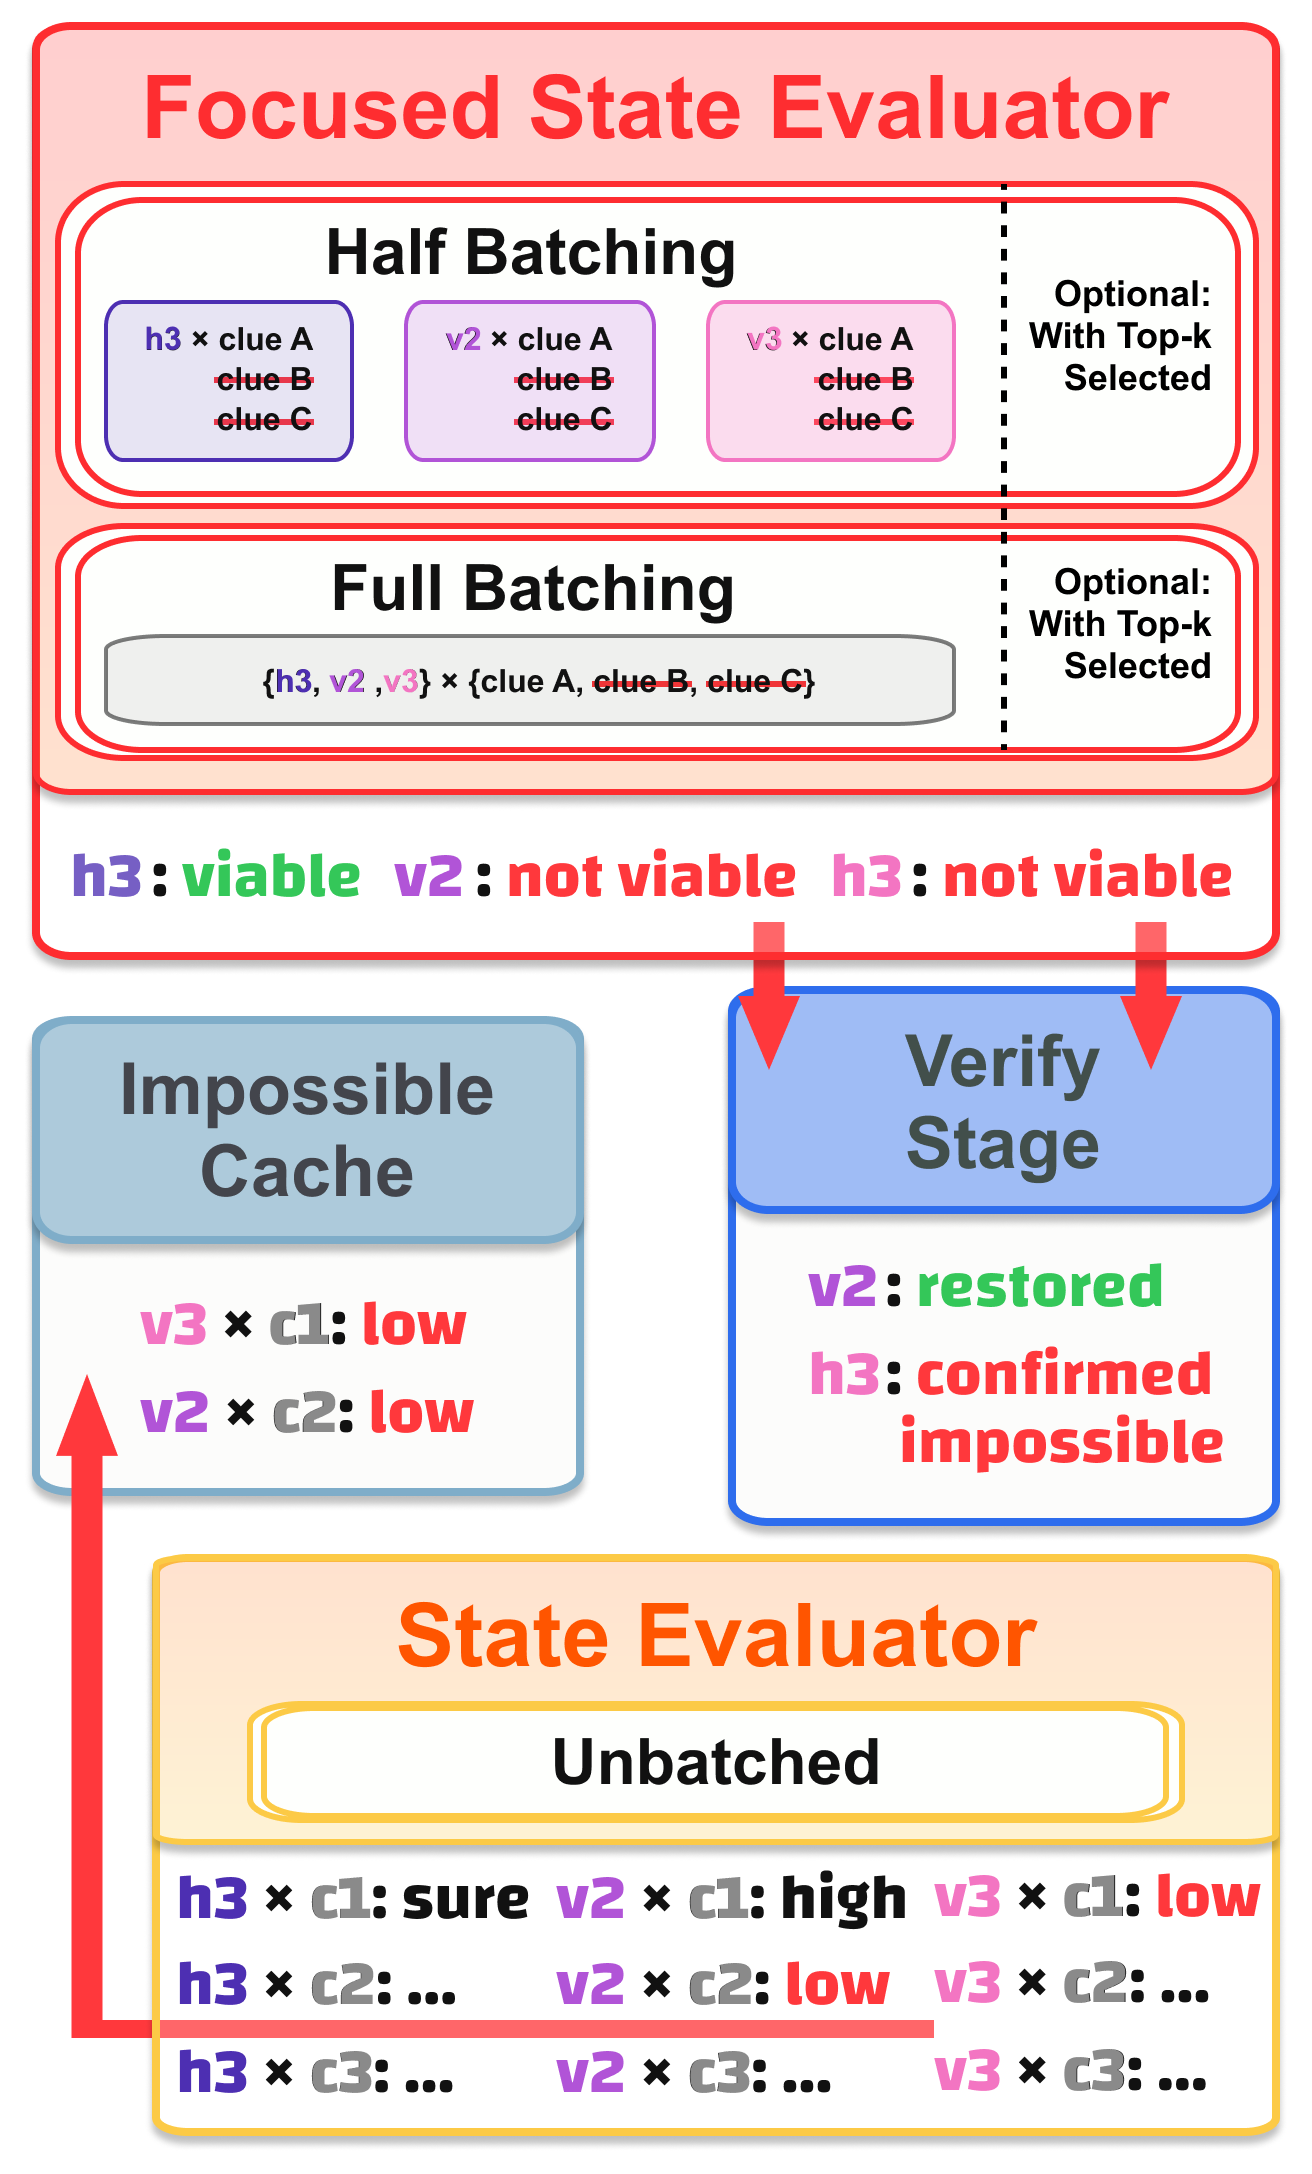
\includegraphics[width=\linewidth]{CW_plots/fig4.png}
\end{minipage}
\vspace{-0.4em}
\heading{Decrease Cost for Unbatched Evaluator}
\vspace{-1.2em}
\begin{minipage}[t]{0.77\linewidth}

\begin{figure}[h]
    \centering
    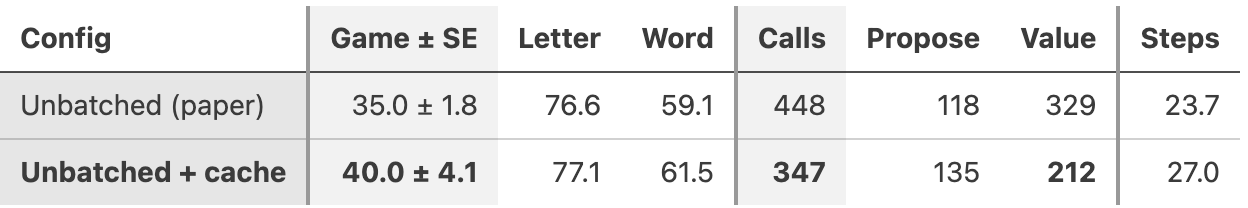
\includegraphics[width=1\linewidth]{CW_plots/fig10.png}
\end{figure}
\end{minipage}
\hfill
\begin{minipage}[t]{0.21\linewidth}
{\footnotesize \textbf{Cache cuts cost without hurting accuracy.}}

\end{minipage}
 

\end{titlelessblock}

\end{column}

\separatorcolumn

% ============================================================
% COLUMN 2 -- Game of 24 (strictly)
% ============================================================
\begin{column}{\colwidth}

\begin{block}{Game of 24: Main Results}
    {\centering
    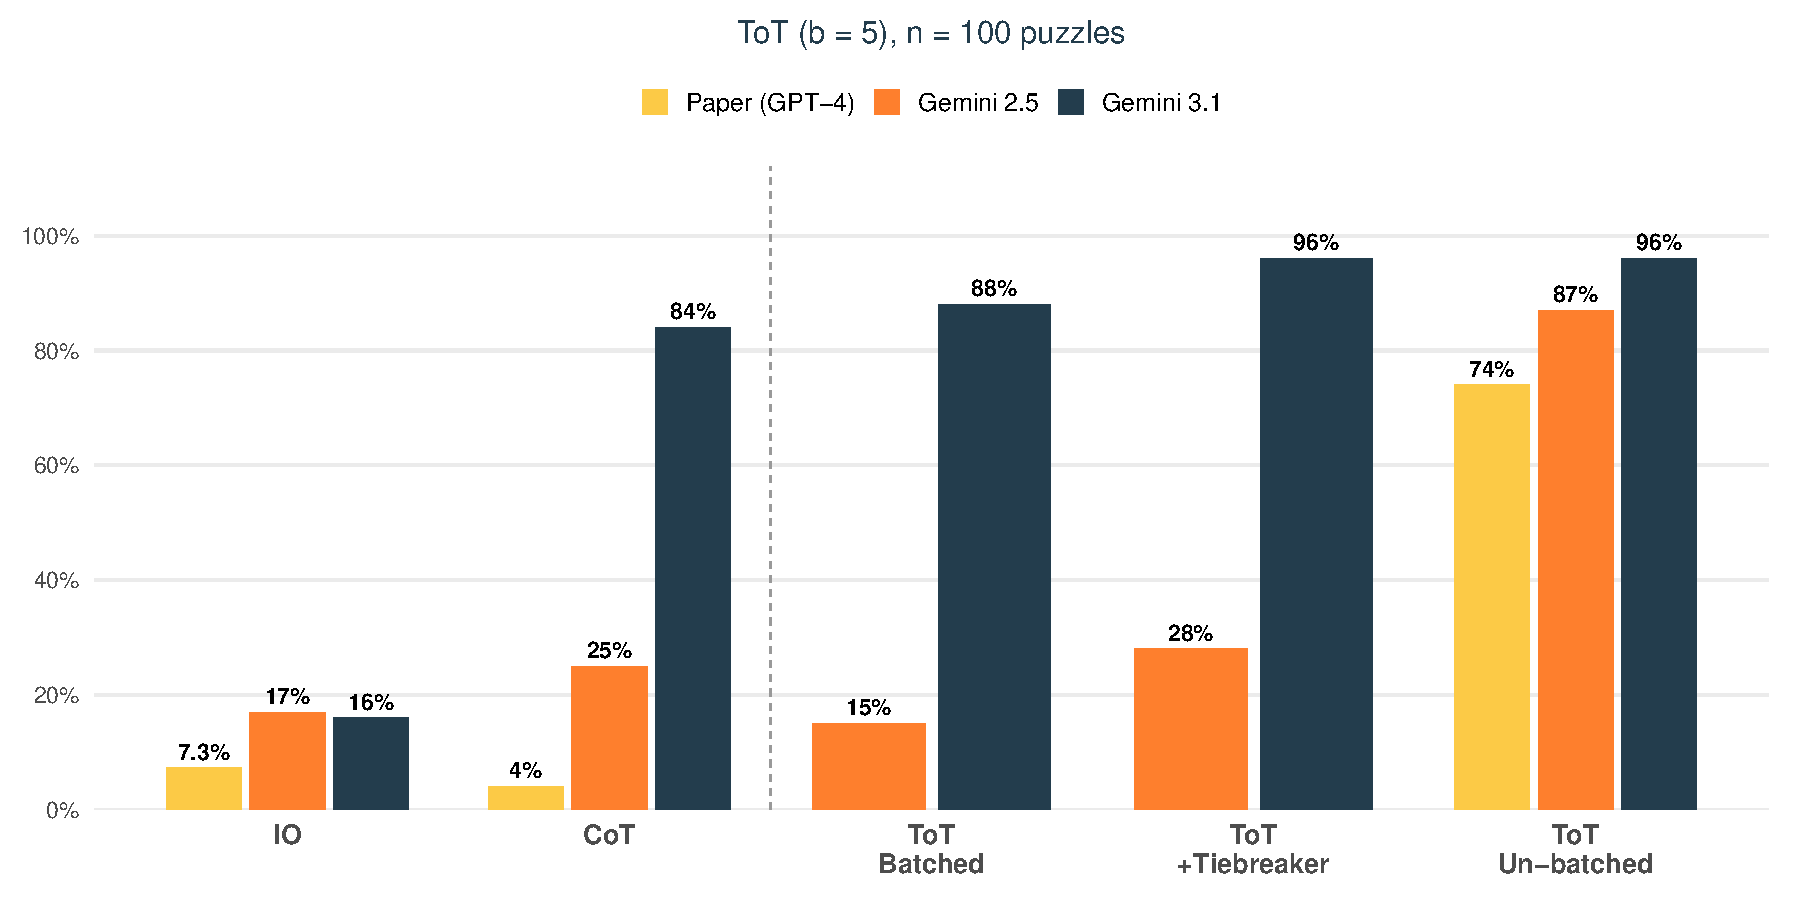
\includegraphics[width=\linewidth]{G24_plots/plot_combined_main.pdf}
    \par}
    \vspace{-0.9em}

    {\small Both Gemini models exceed GPT-4's 74\% with un-batched ToT. Batching hurts Gem~2.5 ($87\%{\to}15\%$) and Gem~3.1 ($96\%{\to}88\%$); the tiebreaker fully recovers Gem~3.1 ($88\%{\to}96\%$) and partially recovers Gem~2.5 ($15\%{\to}28\%$) at zero extra API cost.}
\vspace{-0.3em}
\end{block}

% --- Block 2: Batching Problem ---
\begin{titlelessblock}
\extensionsubtitle{Extension: The Batching Problem}
\begin{minipage}[t]{0.28\linewidth}
\vspace{1.5em}
{\small Un-batching costs ${\sim}3\times$ more but is needed to reproduce the paper.}
\end{minipage}
\hfill
\begin{minipage}[t]{0.70\linewidth}
    \vspace{-1em} {\centering
\footnotesize
\renewcommand{\arraystretch}{1.15}
\begin{tabular}{@{}l r r r@{}}
\toprule
\multicolumn{4}{c}{\textbf{Cost of Un-batching (ToT $b = 5$)}} \\
\midrule
                 & \textbf{Cost / 100} & \textbf{Time / puzzle} & \textbf{API calls} \\
\midrule
\multicolumn{4}{l}{\textit{Gemini 2.5}} \\
\quad Batched    & \$0.32 & ${\sim}8$\,s  & ${\sim}20$  \\
\quad Un-batched & \$0.99 & ${\sim}70$\,s & ${\sim}170$ \\
\midrule
\multicolumn{4}{l}{\textit{Gemini 3.1}} \\
\quad Batched    & \$0.77 & ${\sim}12$\,s & ${\sim}20$  \\
\quad Un-batched & \$3.52 & ${\sim}90$\,s & ${\sim}170$ \\
\bottomrule
\end{tabular}
\par}
\vspace{-0.05em}
\end{minipage}

% --- Sub: Why Batching Hurts ---
\heading{Why Batching Hurts}
    \vspace{-0.23em}
    \begin{figure}
      \centering
      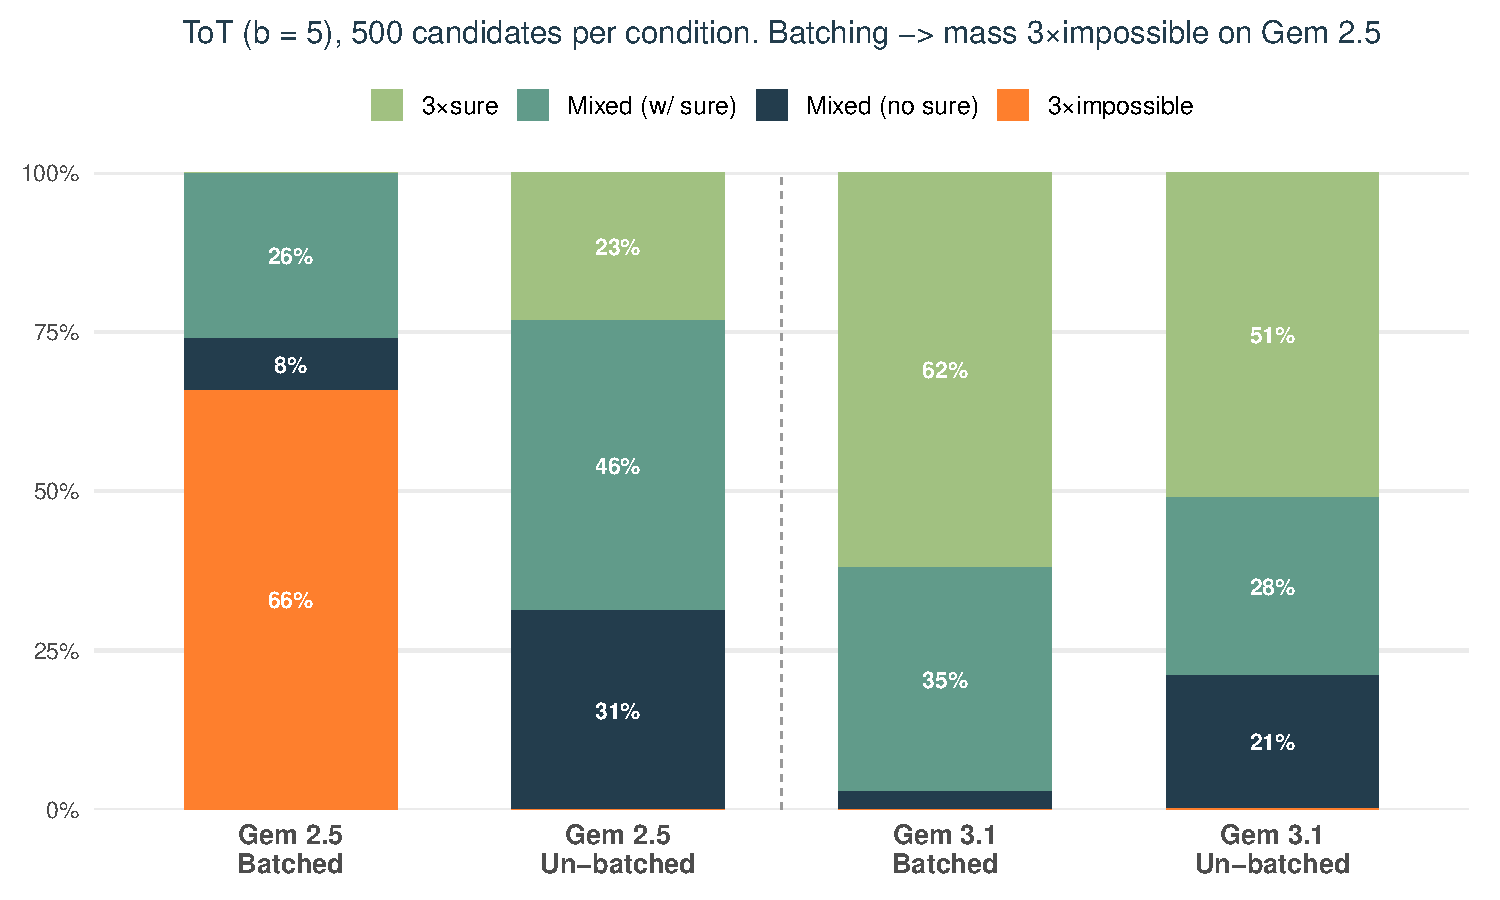
\includegraphics[width=0.7\linewidth]{G24_plots/plot2_verdict_distribution.pdf}
    \end{figure}
    \vspace{-0.8em}
    {\small Batched Gem~2.5 votes "impossible" on 66\%of depth-0 candidates (vs.\ 0\% un-batched). Gem~3.1 resists: 62\% ``sure'' when batched.}

\vspace{-0.2em}
% --- Sub: Verifier Tiebreaker ---
\heading{Verifier Tiebreaker}
    \vspace{-0.5em}
    \begin{figure}
      \centering
      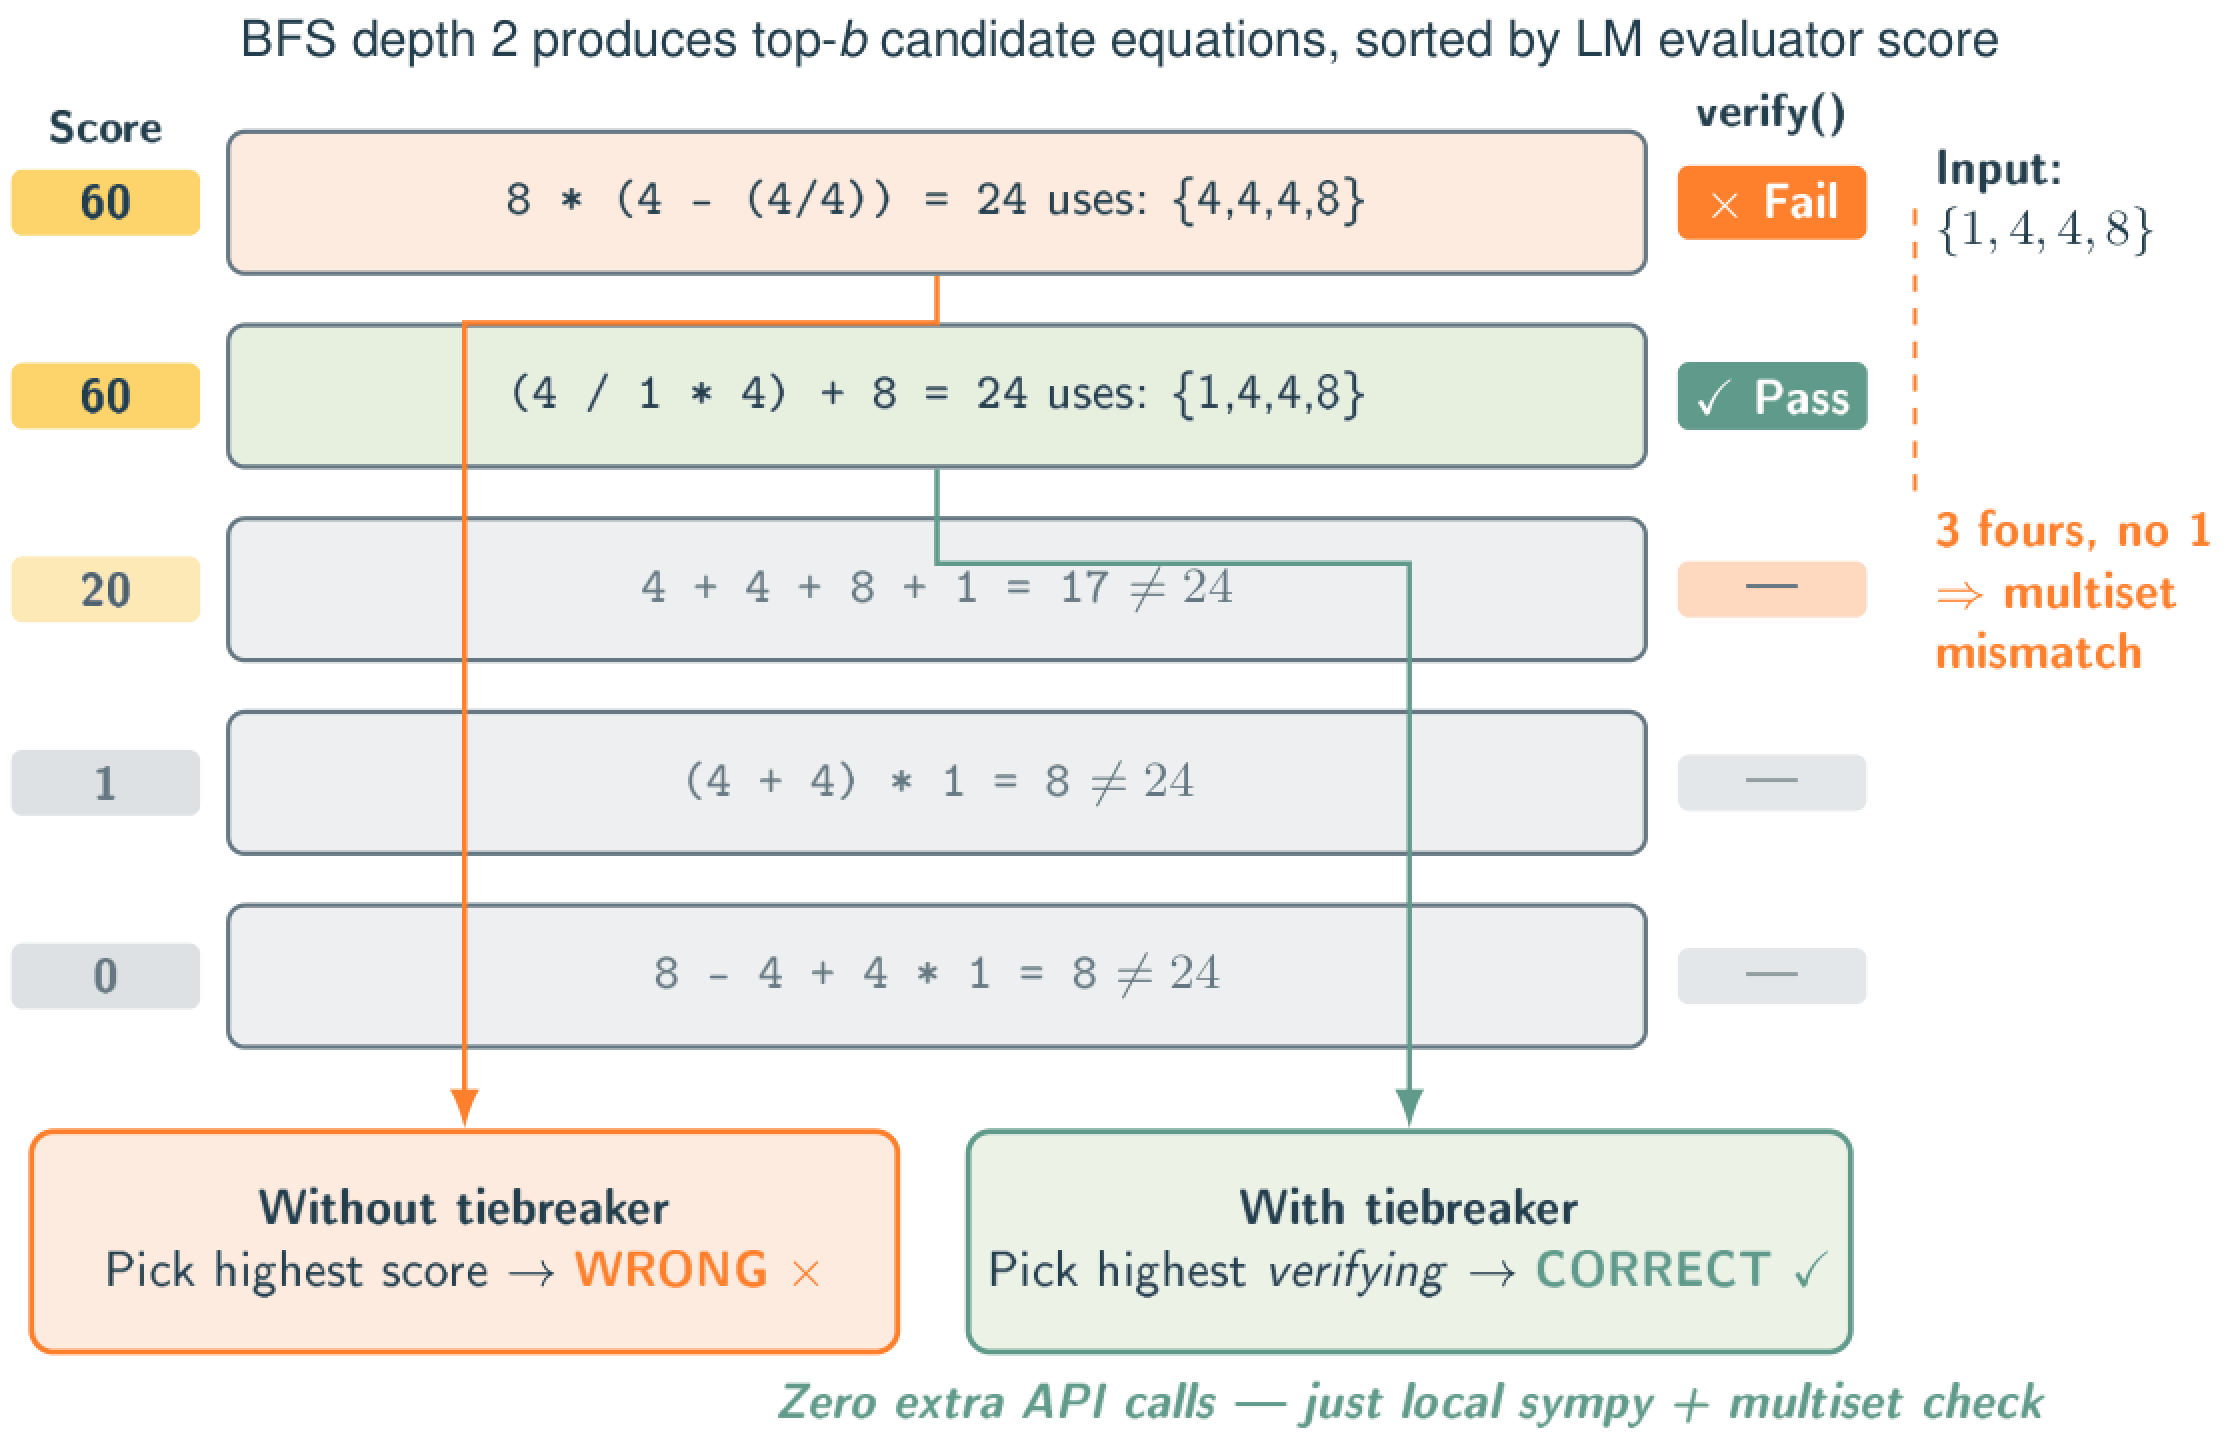
\includegraphics[width=1\linewidth]{G24_plots/tiebreaker_diagram.png}
    \end{figure}
  \end{titlelessblock}
\end{column}
\separatorcolumn


% ============================================================
% COLUMN 4 -- Creative Writing 
% ============================================================
\begin{column}{\colwidth}

\begin{block}{Creative Writing}
\vspace{-0.8em}

\heading{Main baselines + Refinement}
    \vspace{-0.5em}
\small{Across IO, CoT, and ToT, compare the baseline with addition of a post-generation revision step.}

    \vspace{-0.5em}
    \begin{figure}
      \centering
      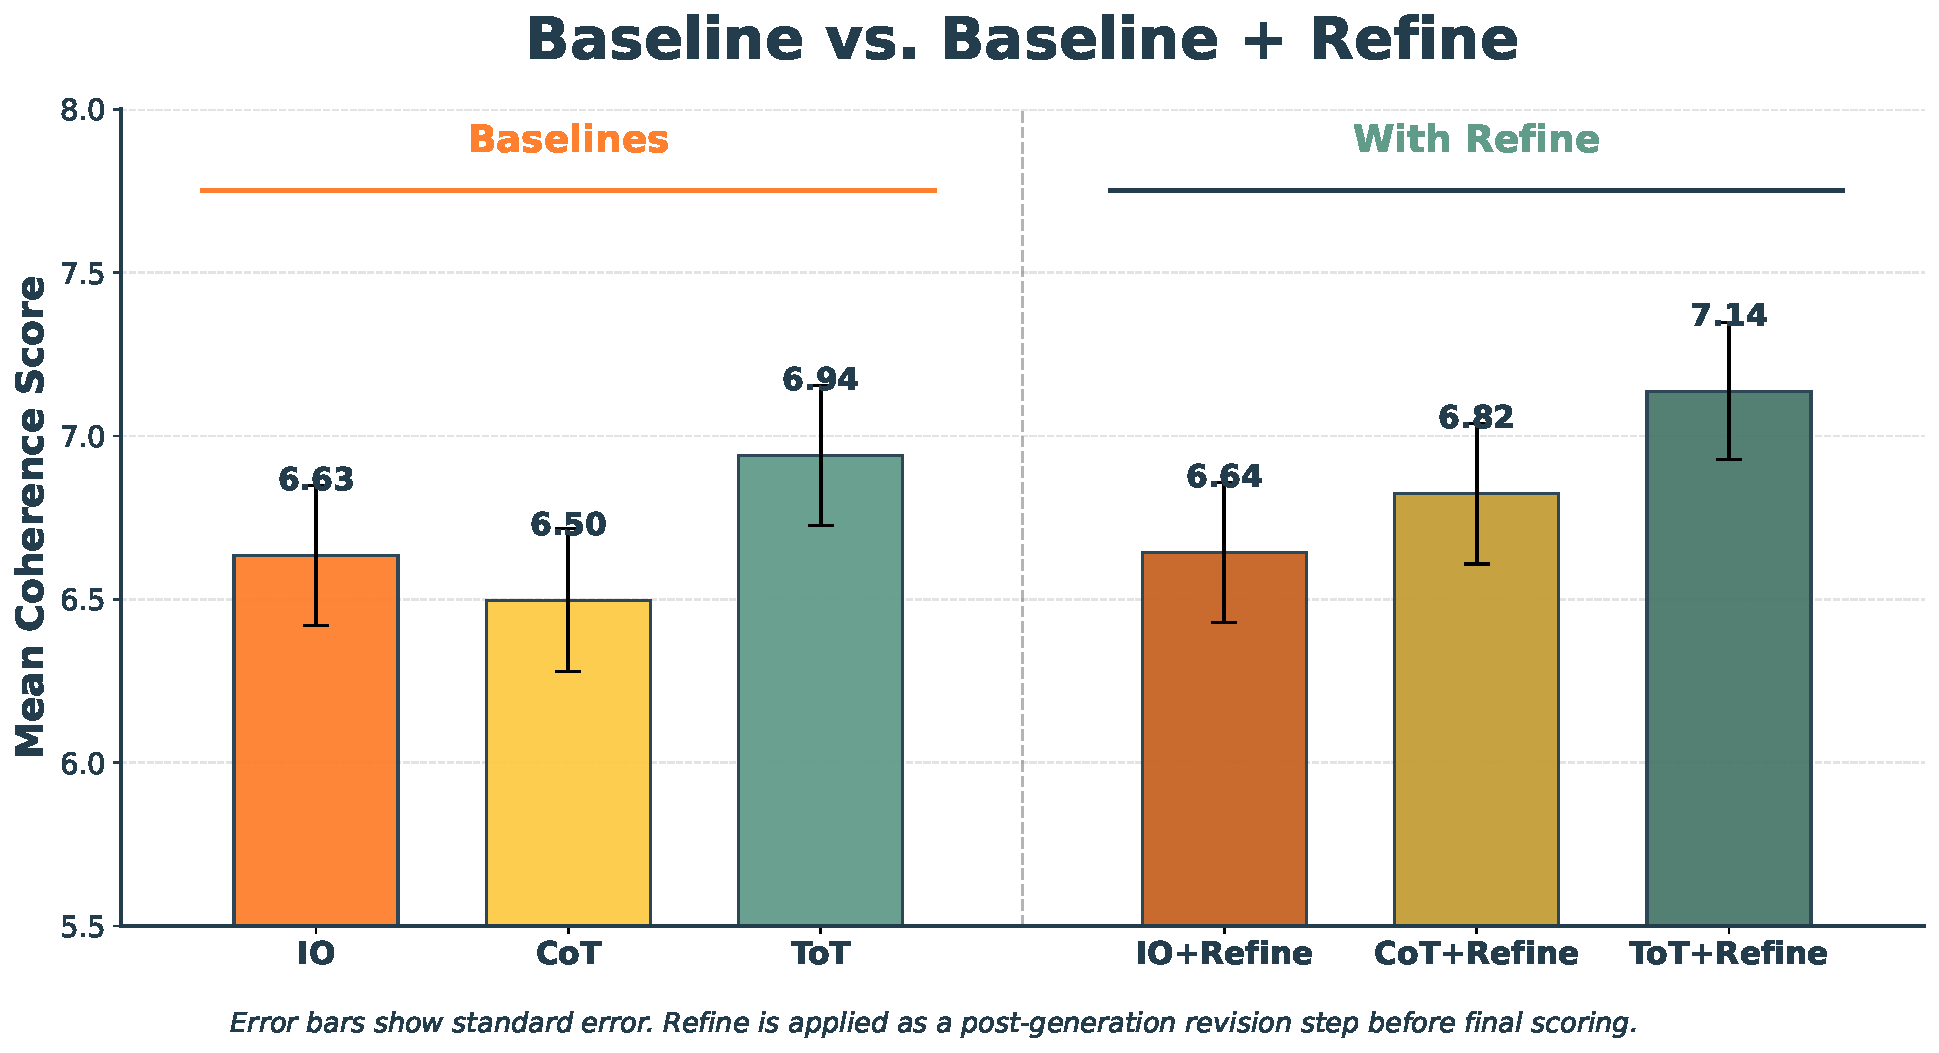
\includegraphics[width=0.85\linewidth]{Text_plots/cw_fig1.pdf}
    \end{figure}
    \vspace{-0.8em}


\end{block}

% --- Block 2: Extension ---
\begin{titlelessblock}
\extensionsubtitle{Extension: Isolate Selection vs Sampling Effects}


    \vspace{-0.4em}
    \begin{figure}
      \centering
      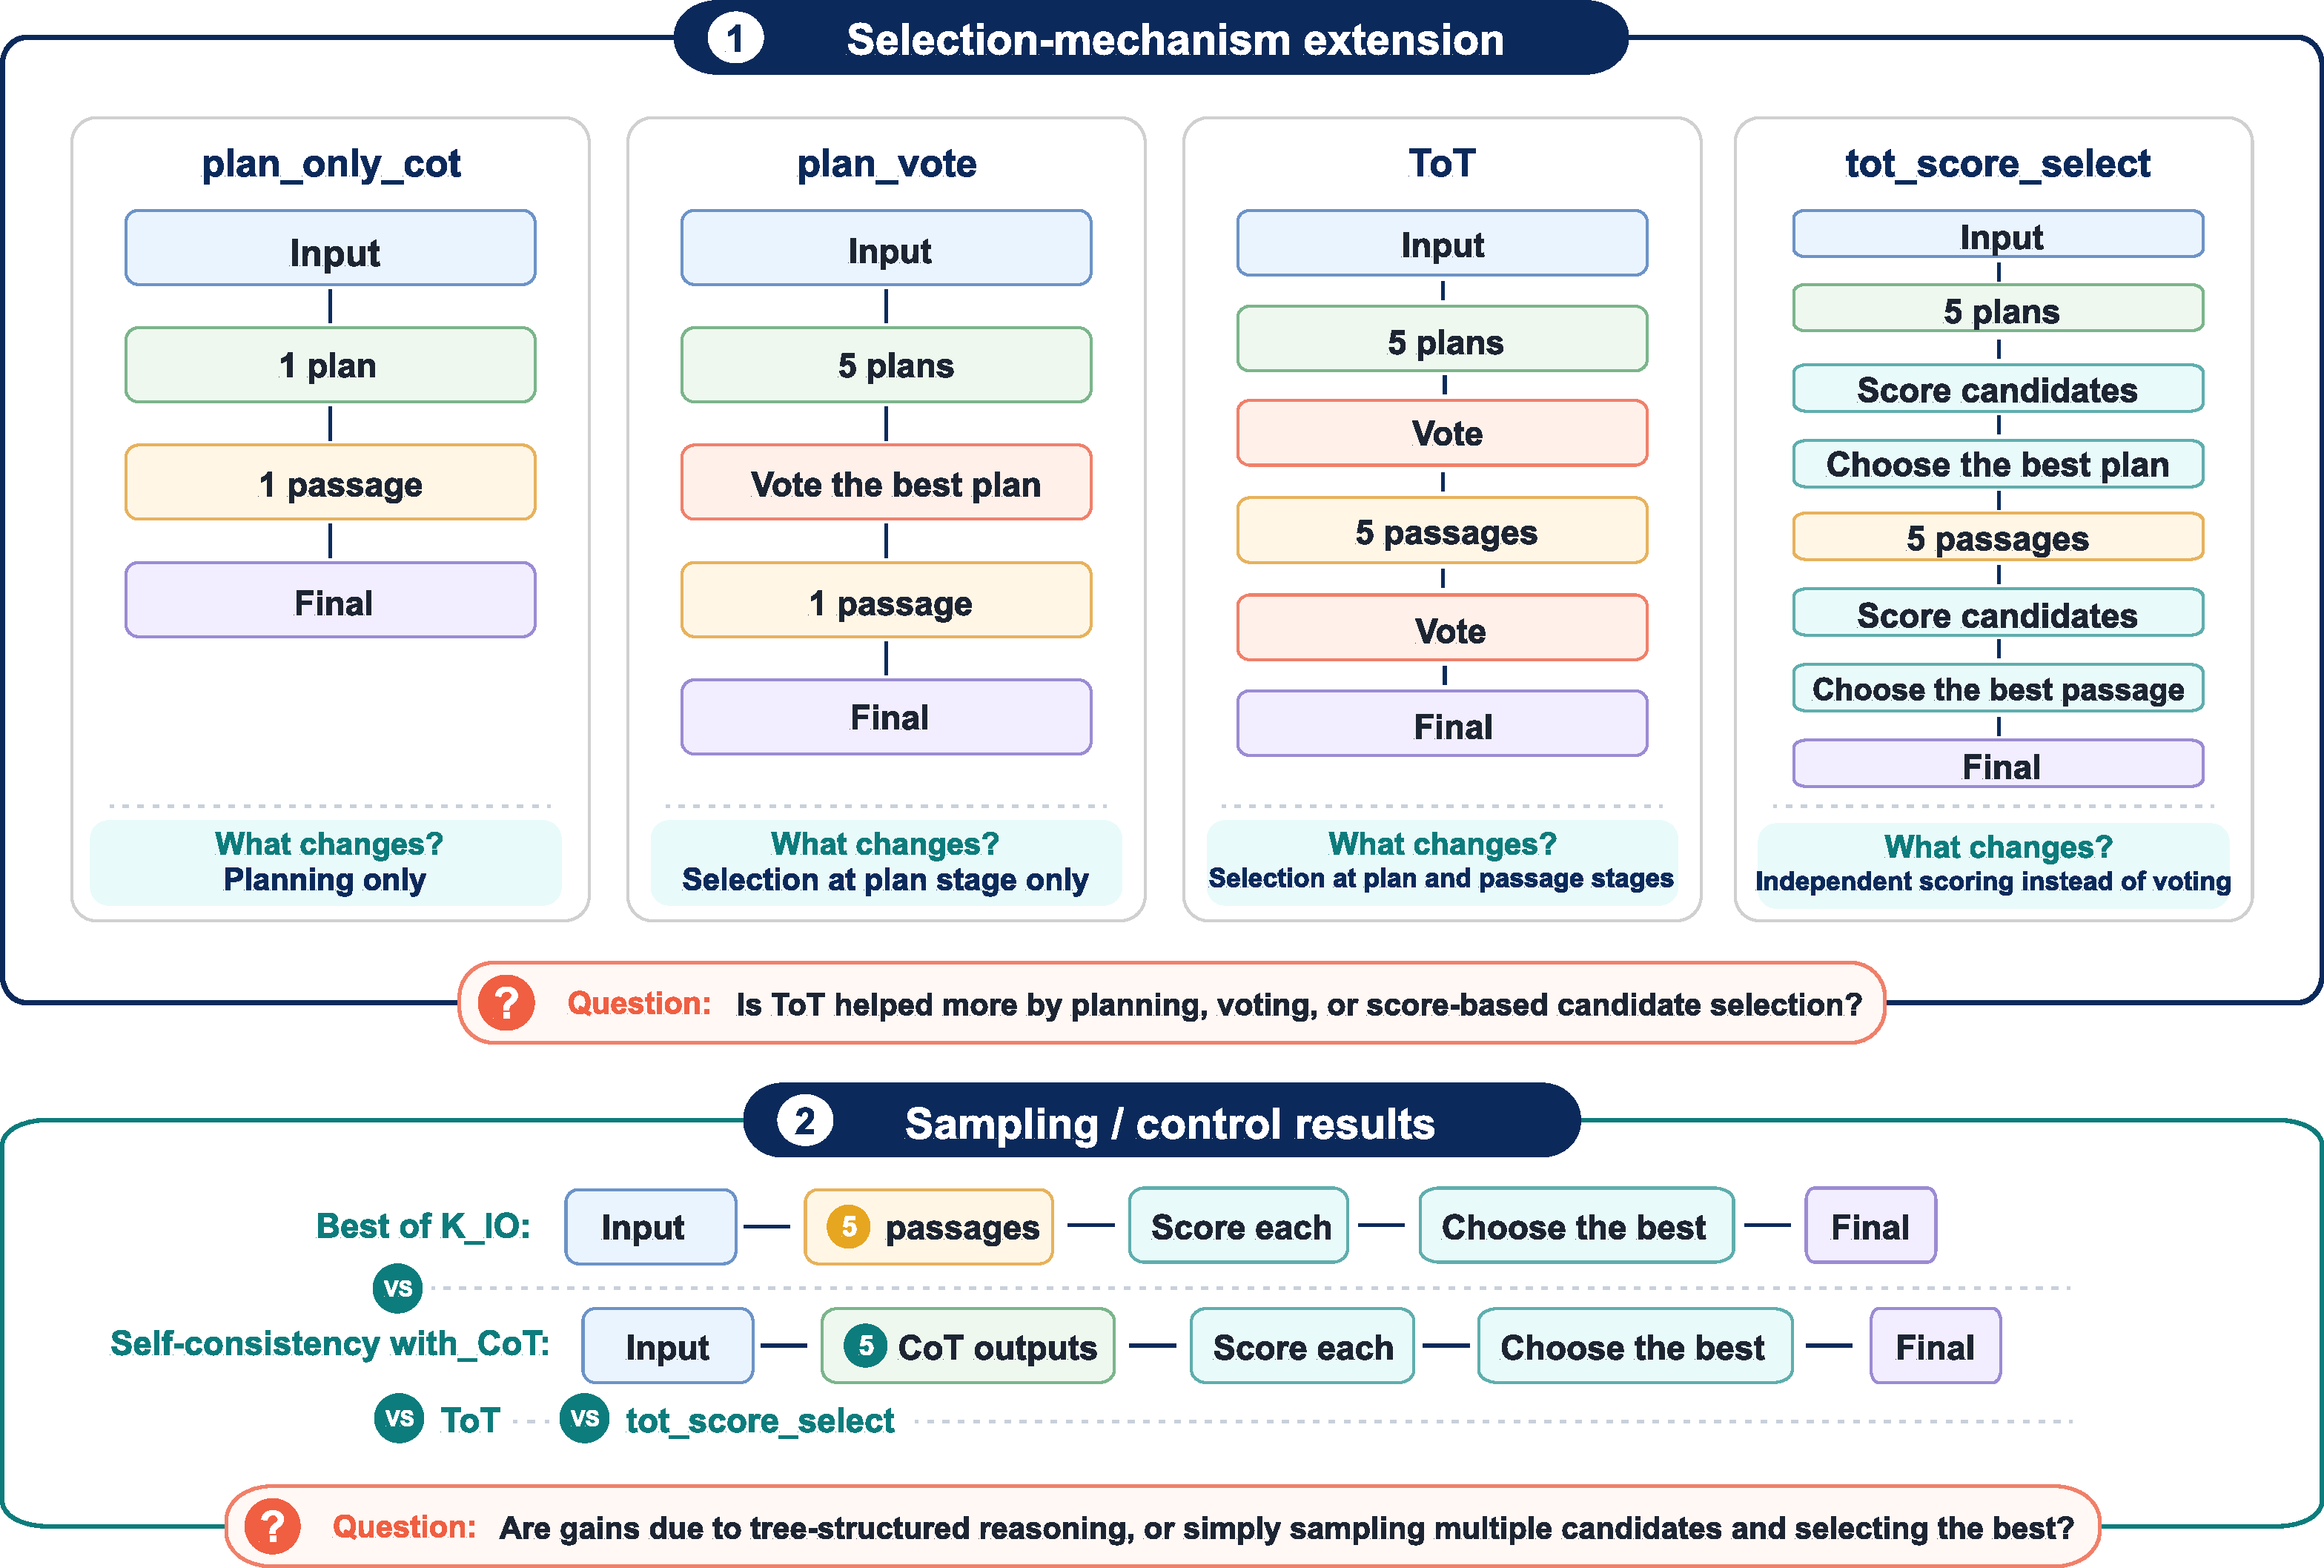
\includegraphics[width=1.0\linewidth]{Text_plots/cw_fig2.pdf}
    \end{figure}
    \vspace{-0.em}

\small{
\textbf{ToT score-select} achieves the highest mean coherence score (8.14), with scores more concentrated near the top range. \\
\textbf{Best-of-k IO and self-consistency with CoT} also outperform standard ToT, suggesting that sampling multiple candidates is a strong baseline. \\

}

\vspace{0.8em}
    \begin{minipage}[t]{0.48\linewidth}
      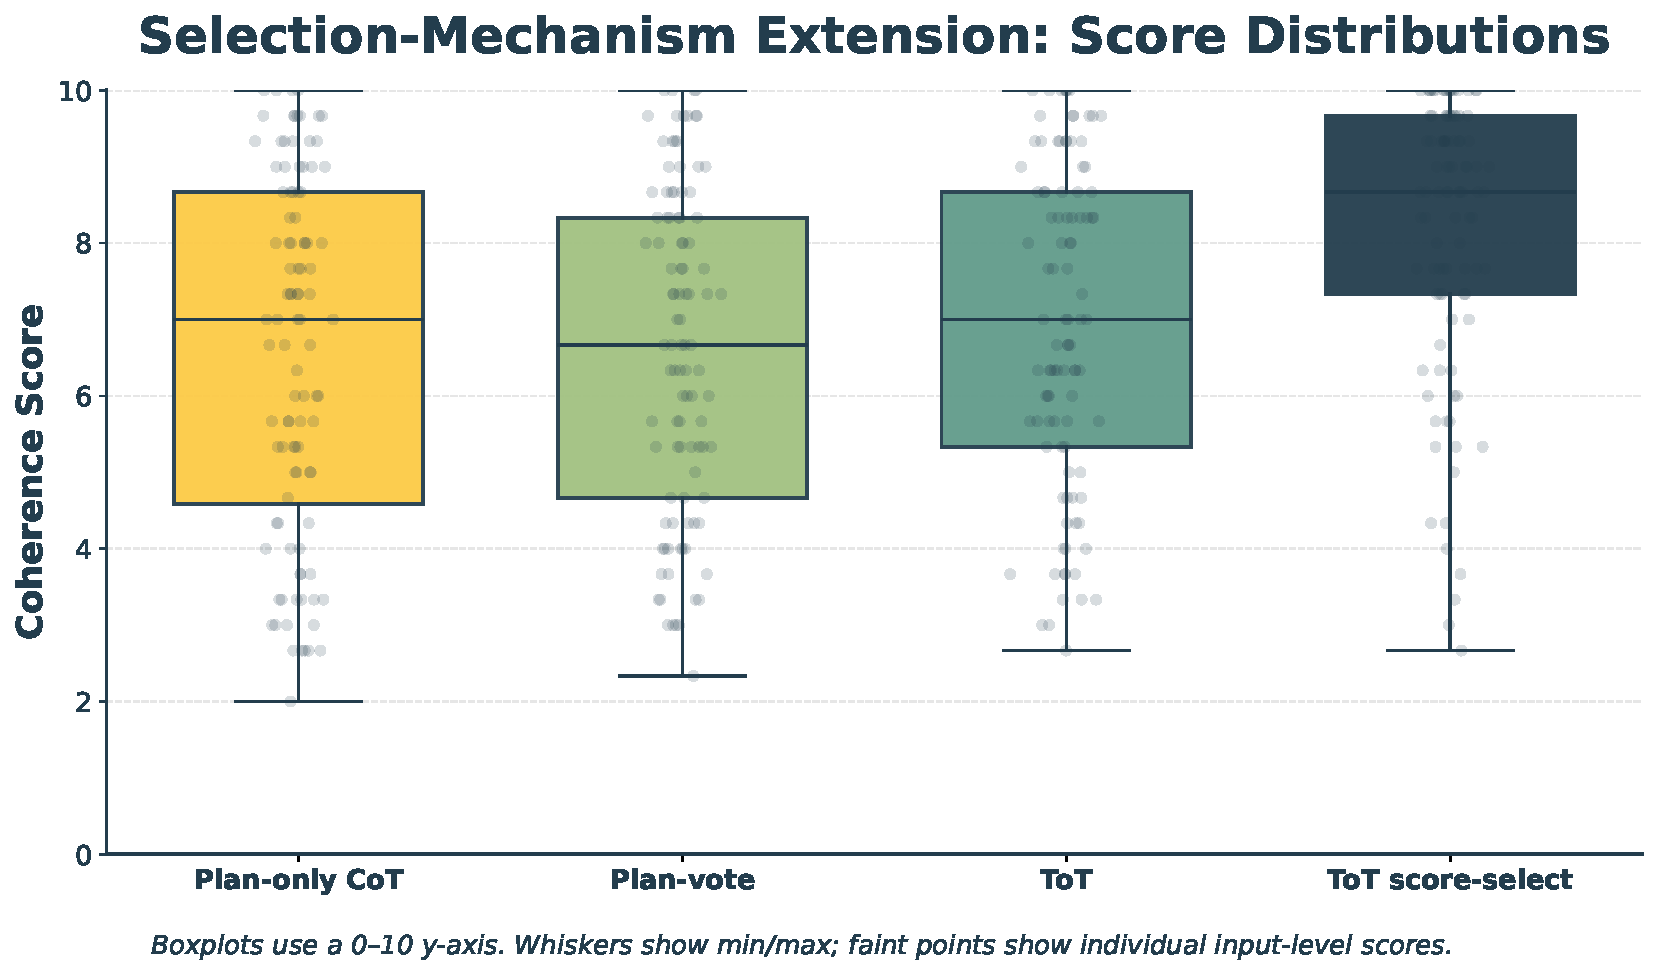
\includegraphics[width=\linewidth]{Text_plots/cw_fig3.pdf}
    \end{minipage}%
    \hfill
    \begin{minipage}[t]{0.48\linewidth}
      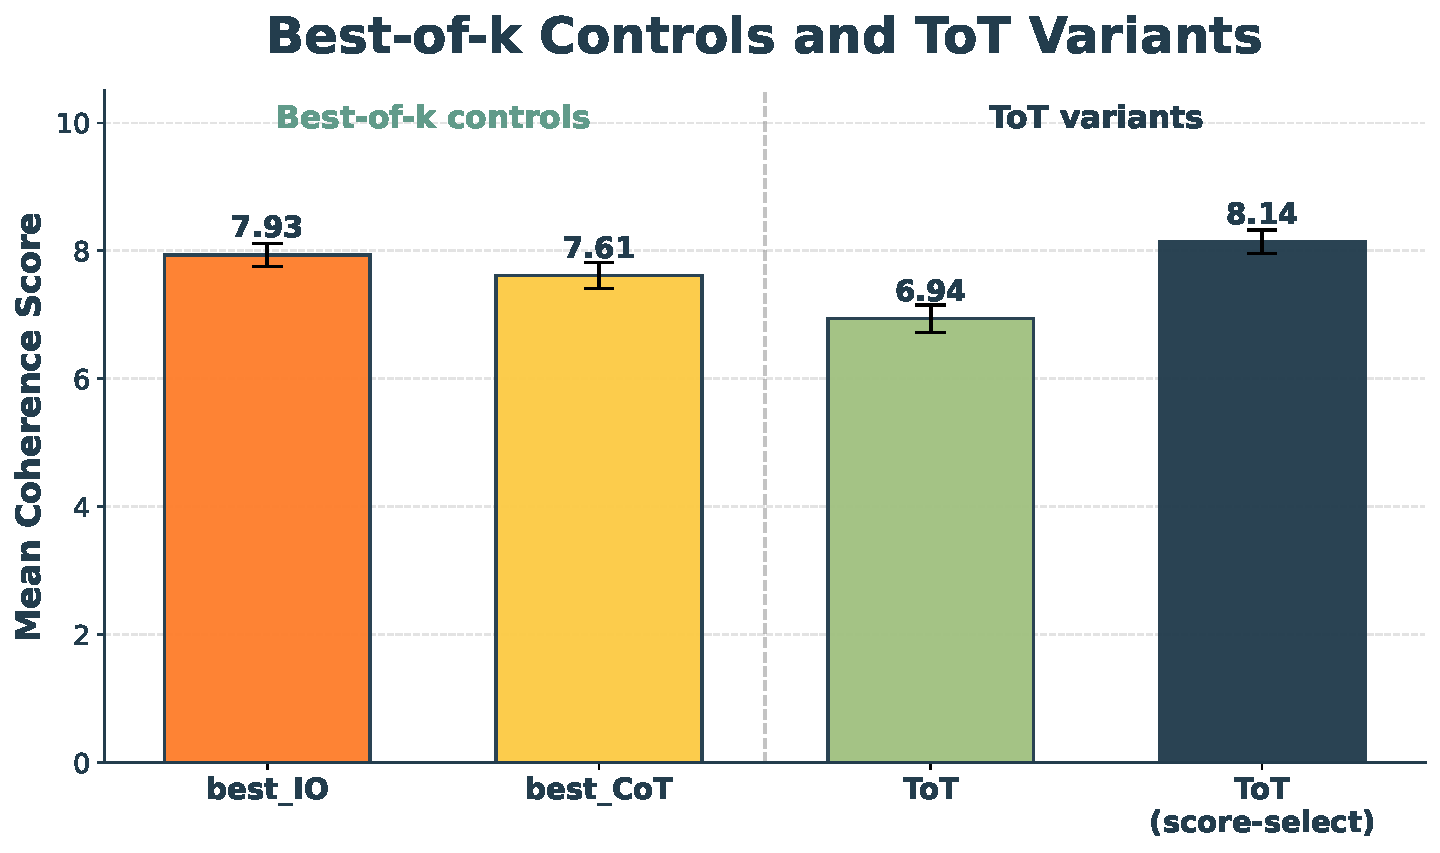
\includegraphics[width=\linewidth]{Text_plots/cw_fig4.pdf}
    \end{minipage}%

\vspace{-0.05em}
\small{The main gain appears to come from candidate scoring/selection rather than standard vote-based ToT.}

\vspace{1.0em}
  \end{titlelessblock}



\begin{block}{Conclusions}
\vspace{-0.6em}
\small{
\begin{itemize}
    \item \textbf{ToT's gains replicate} on 2026 models without batching.
    %
    \item \textbf{Batching silently breaks ToT} across applicable tasks, i.e.\ Game of 24 and Crosswords, whether with Gem 2.5 or Gem 3.1. Remedial strategies close the accuracy gap for Gem 3.1.
    %
    \item \textbf{For Creative Writing,} ToT benefits less from voting and more from strong candidate selection (score-based selection outperforms standard vote-based ToT).
\end{itemize}
}
\end{block}

\end{column}

\separatorcolumn

\end{columns}


% ============================================================
% FIXED BOTTOM REFERENCES BAR
% Uses \hfill-separated minipages instead of beamer's \begin{columns},
% which can collapse / fail to render when nested inside a TikZ node.
% Anchor moved up (yshift=0.4in) so the body has clearance from the page edge.
% ============================================================
\begin{tikzpicture}[remember picture,overlay]
\node[
  anchor=south west,
  inner sep=0pt
] at ([xshift=0.45in,yshift=0.4in]current page.south west) {%
  \begin{minipage}{35.1in}
    \begin{beamercolorbox}[
      wd=\linewidth,
      ht=0.7cm,
      dp=0.18cm,
      center
    ]{block title}
      \textbf{References}
    \end{beamercolorbox}

    \begin{beamercolorbox}[
      wd=\linewidth,
      sep=0.15cm
    ]{block body}
      \begin{minipage}[t]{0.30\linewidth}
        {\scriptsize
          \textbf{[1]} Shunyu Yao et al.\
          \textit{Tree of Thoughts: Deliberate Problem Solving with Large Language Models}.
          NeurIPS, 2023.
        }
      \end{minipage}\hfill
      \begin{minipage}[t]{0.42\linewidth}
        {\scriptsize
          \textbf{[2]} Zhoujun Cheng, Jungo Kasai, and Tao Yu.
          \textit{Batch Prompting: Efficient Inference with Large Language Model APIs}.
          EMNLP Industry Track, 2023.
        }
      \end{minipage}\hfill
      \begin{minipage}[t]{0.22\linewidth}
        {\scriptsize
          \textbf{[3]} Jianzhe Lin et al.\
          \textit{BatchPrompt: Accomplish More with Less}.
          ICLR, 2024.
        }
      \end{minipage}
    \end{beamercolorbox}
  \end{minipage}
};
\end{tikzpicture}

\end{frame}
\end{document}